%!TEX program = xelatex
\documentclass[a4paper,12pt]{report}
\usepackage{indentfirst} 
\usepackage{ctex}
%\usepackage{xeCJK}
\usepackage{times}
\usepackage{graphicx,float}
\usepackage{subcaption}
\usepackage{setspace}
\usepackage{fancyhdr}
% \usepackage{graphicx}
\usepackage{wrapfig}
\usepackage{array}
\usepackage{fontspec,xunicode,xltxtra}
\usepackage{titlesec}
\usepackage{titletoc}
\usepackage[titletoc]{appendix}
\usepackage[top=30mm,bottom=30mm,left=20mm,right=20mm]{geometry}
\usepackage{cite}
\usepackage{listings}
\usepackage{hyperref}
\usepackage[framed,numbered,autolinebreaks,useliterate]{mcode} % 插入代码
\XeTeXlinebreaklocale "zh"
\XeTeXlinebreakskip = 0pt plus 1pt minus 0.1pt

%---------------------------------------------------------------------
%	页眉页脚设置
%---------------------------------------------------------------------
\fancypagestyle{plain}{
	\pagestyle{fancy}      %改变章节首页页眉
}

\pagestyle{fancy}
\lhead{\kaishu~``软件测试与维护''实验报告~}
\rhead{\kaishu~~大作业实验报告}
\cfoot{\thepage}

%---------------------------------------------------------------------
%	章节标题设置
%---------------------------------------------------------------------
\titleformat{\chapter}{\centering\zihao{-1}\heiti}{实验\chinese{chapter}}{1em}{}
\titlespacing{\chapter}{0pt}{*0}{*6}

%---------------------------------------------------------------------
%	摘要标题设置
%---------------------------------------------------------------------
\renewcommand{\abstractname}{\zihao{-3} 摘\quad 要}

%---------------------------------------------------------------------
%	参考文献设置
%---------------------------------------------------------------------
\renewcommand{\bibname}{\zihao{2}{\hspace{\fill}参\hspace{0.5em}考\hspace{0.5em}文\hspace{0.5em}献\hspace{\fill}}}

%---------------------------------------------------------------------
%	引用文献设置为上标
%---------------------------------------------------------------------
\makeatletter
\def\@cite#1#2{\textsuperscript{[{#1\if@tempswa , #2\fi}]}}
\makeatother

%---------------------------------------------------------------------
%	目录页设置
%---------------------------------------------------------------------
\titlecontents{chapter}[0em]{\songti\zihao{-4}}{\thecontentslabel\ }{}
{\hspace{.5em}\titlerule*[4pt]{$\cdot$}\contentspage}
\titlecontents{section}[2em]{\vspace{0.1\baselineskip}\songti\zihao{-4}}{\thecontentslabel\ }{}
{\hspace{.5em}\titlerule*[4pt]{$\cdot$}\contentspage}
\titlecontents{subsection}[4em]{\vspace{0.1\baselineskip}\songti\zihao{-4}}{\thecontentslabel\ }{}
{\hspace{.5em}\titlerule*[4pt]{$\cdot$}\contentspage}

\renewcommand\thesection{\arabic{section}}
\renewcommand\thesubsection{\arabic{section}.\arabic{subsection}}

\begin{document}
%---------------------------------------------------------------------
%	封面设置
%---------------------------------------------------------------------
\begin{titlepage}
	\begin{center}
		
    
\includegraphics[width=1.0\textwidth]{figure//nankai.jpg}\\
    % \vspace{10mm}
    % \textbf{\zihao{2}\kaishu{软件学院}}\\[0.8cm]
    \vspace{50mm}
    \textbf{\zihao{1}\heiti{ 《软件测试与维护》实验报告}}\\[1cm]
    \textbf{\zihao{2}\heiti{ (2025\textasciitilde2026学年第二学期)}}\\[1cm]
    %\textbf{\zihao{2}\heiti{ 实验1: Wireshark软件使用与ARP协议分析}}\\[2cm]
	\vspace{\fill}
	
\setlength{\extrarowheight}{2mm}
{\songti\zihao{3}	
\begin{tabular}{rl}

	{\makebox[4\ccwd][s]{实验名称：}}& ~\kaishu 软件测试与维护大作业\\
	{\makebox[4\ccwd][s]{学\qquad 院：}}& ~\kaishu 软件学院\\
		{\makebox[4\ccwd][s]{姓\qquad 名：}}& ~\kaishu 第九组\\

	{\makebox[4\ccwd][s]{指导老师：}} & ~\kaishu 张圣林\\

\end{tabular}
 }\\[2cm]
\vspace{\fill}
\zihao{4}
%2023\textasciitilde 2023秋季学期\\
%使用\LaTeX 撰写于
    \today
	\end{center}	
\end{titlepage}


%---------------------------------------------------------------------
%  目录页
%---------------------------------------------------------------------
\tableofcontents % 生成目录

%---------------------------------------------------------------------
%  实验一
%---------------------------------------------------------------------
\chapter*{软件测试与维护大作业}
\setcounter{page}{1}
\begin{spacing}{1.5}
\songti\zihao{-4}

\section{分工情况与项目概述}
\subsection*{分工情况}
    \begin{center}
    \begin{table*}[h]
        \centering
        \renewcommand{\arraystretch}{1.5}  % 增加行高，使内容更舒适
        \begin{tabular}{|c|c|c|}  % 列数改为3列
            \hline
            \textbf{学号} & \textbf{姓名} & \textbf{    主要分工    } \\
            \hline
            2311189 & 兰子毅 & 
            \begin{minipage}[t]{12cm}
               在已有微服务系统的基础上增加inventory和restock两个微服务
            \end{minipage} \\
            \hline
            2312454 & 张乐 & 
            \begin{minipage}[t]{12cm}
                部署、故障注入与监控、指标数据采集分析、指标论文复现
            \end{minipage} \\
            \hline
            2311269 & 孙威旺 & 
            \begin{minipage}[t]{12cm}
                对微服务进行测试，生成论文复现用数据集，复现LogRobust，协助完成论文对比实验
            \end{minipage} \\
            \hline
            2312432 & 方言 & 
            \begin{minipage}[t]{12cm}
                复现Lightlog并对其进行消融测试，复现LogAnomaly，并进行LightLog与其他论文的对比实验
            \end{minipage} \\
            \hline
            2312330 & 赵文卓 & 
            \begin{minipage}[t]{12cm}
                运维智能体前后端、命令行端全部开发、运行、测试
            \end{minipage} \\
            \hline
        \end{tabular}
        \caption{小组成员分工表（排名不分先后，按报告负责顺序）}
        \label{tab:team_division}
    \end{table*}
\end{center}

\subsection*{项目概述}

本项目基于Minikube Kubernetes 集群与 Docker 容器化技术，完成了完整的微服务部
署、自动化测试、监控运维与异常检测全流程实验。

项目部署Online-Boutique开源微服务集
群，搭配PrometheusGrafana 搭建监控体系，利用ChaosMesh注入各类故障，通过Selenium、
JMeter 分别完成系统功能自动化测试与性能压力测试，用采集的真实运维测试数据复现多篇论文
并进行多种实验。

项目为Online-Boutique开源微服务新开发两个微服务，扩展了其功能。

项目开发一个新型智能体以完成智能化运维任务。

项目源码仓库链接：\url{https://github.com/darkness650/ops_test_lastHomework.git}

本报告各部分由相应分工部分同学完成

\section{微服务系统介绍和开发}

本部分工作基于 Google Cloud 的 Online Boutique 微服务示例系统进行扩展。原系统已经具备商品浏览、购物车、结算、推荐、广告、支付、邮件、配送等典型电商功能，能够体现多语言、多服务协同工作的微服务架构特点。但是，原项目的商品购买流程并没有真正维护库存状态：用户可以反复加入商品，系统不会判断剩余库存是否足够；清空购物车也不会恢复库存；管理员也没有独立的进货入口。因此，本次开发选择围绕“库存管理”和“进货管理”补充业务能力，在原有系统上新增两个微服务，并对前端服务进行集成改造。

\subsection*{原系统结构}

Online Boutique 原始系统以 \texttt{frontend} 作为用户入口，浏览器和压测程序都通过 HTTP 访问前端服务，再由前端服务调用内部微服务完成页面展示和业务处理。原系统中，\texttt{productcatalogservice} 负责商品数据，\texttt{cartservice} 负责购物车，\texttt{checkoutservice} 负责结算编排，\texttt{currencyservice}、\texttt{paymentservice}、\texttt{shippingservice}、\texttt{emailservice} 等服务分别承担货币换算、支付、配送和邮件通知等职责。整体结构如图 \ref{fig:origin_microservice_arch} 所示。

\begin{figure}[H]
	\centering
	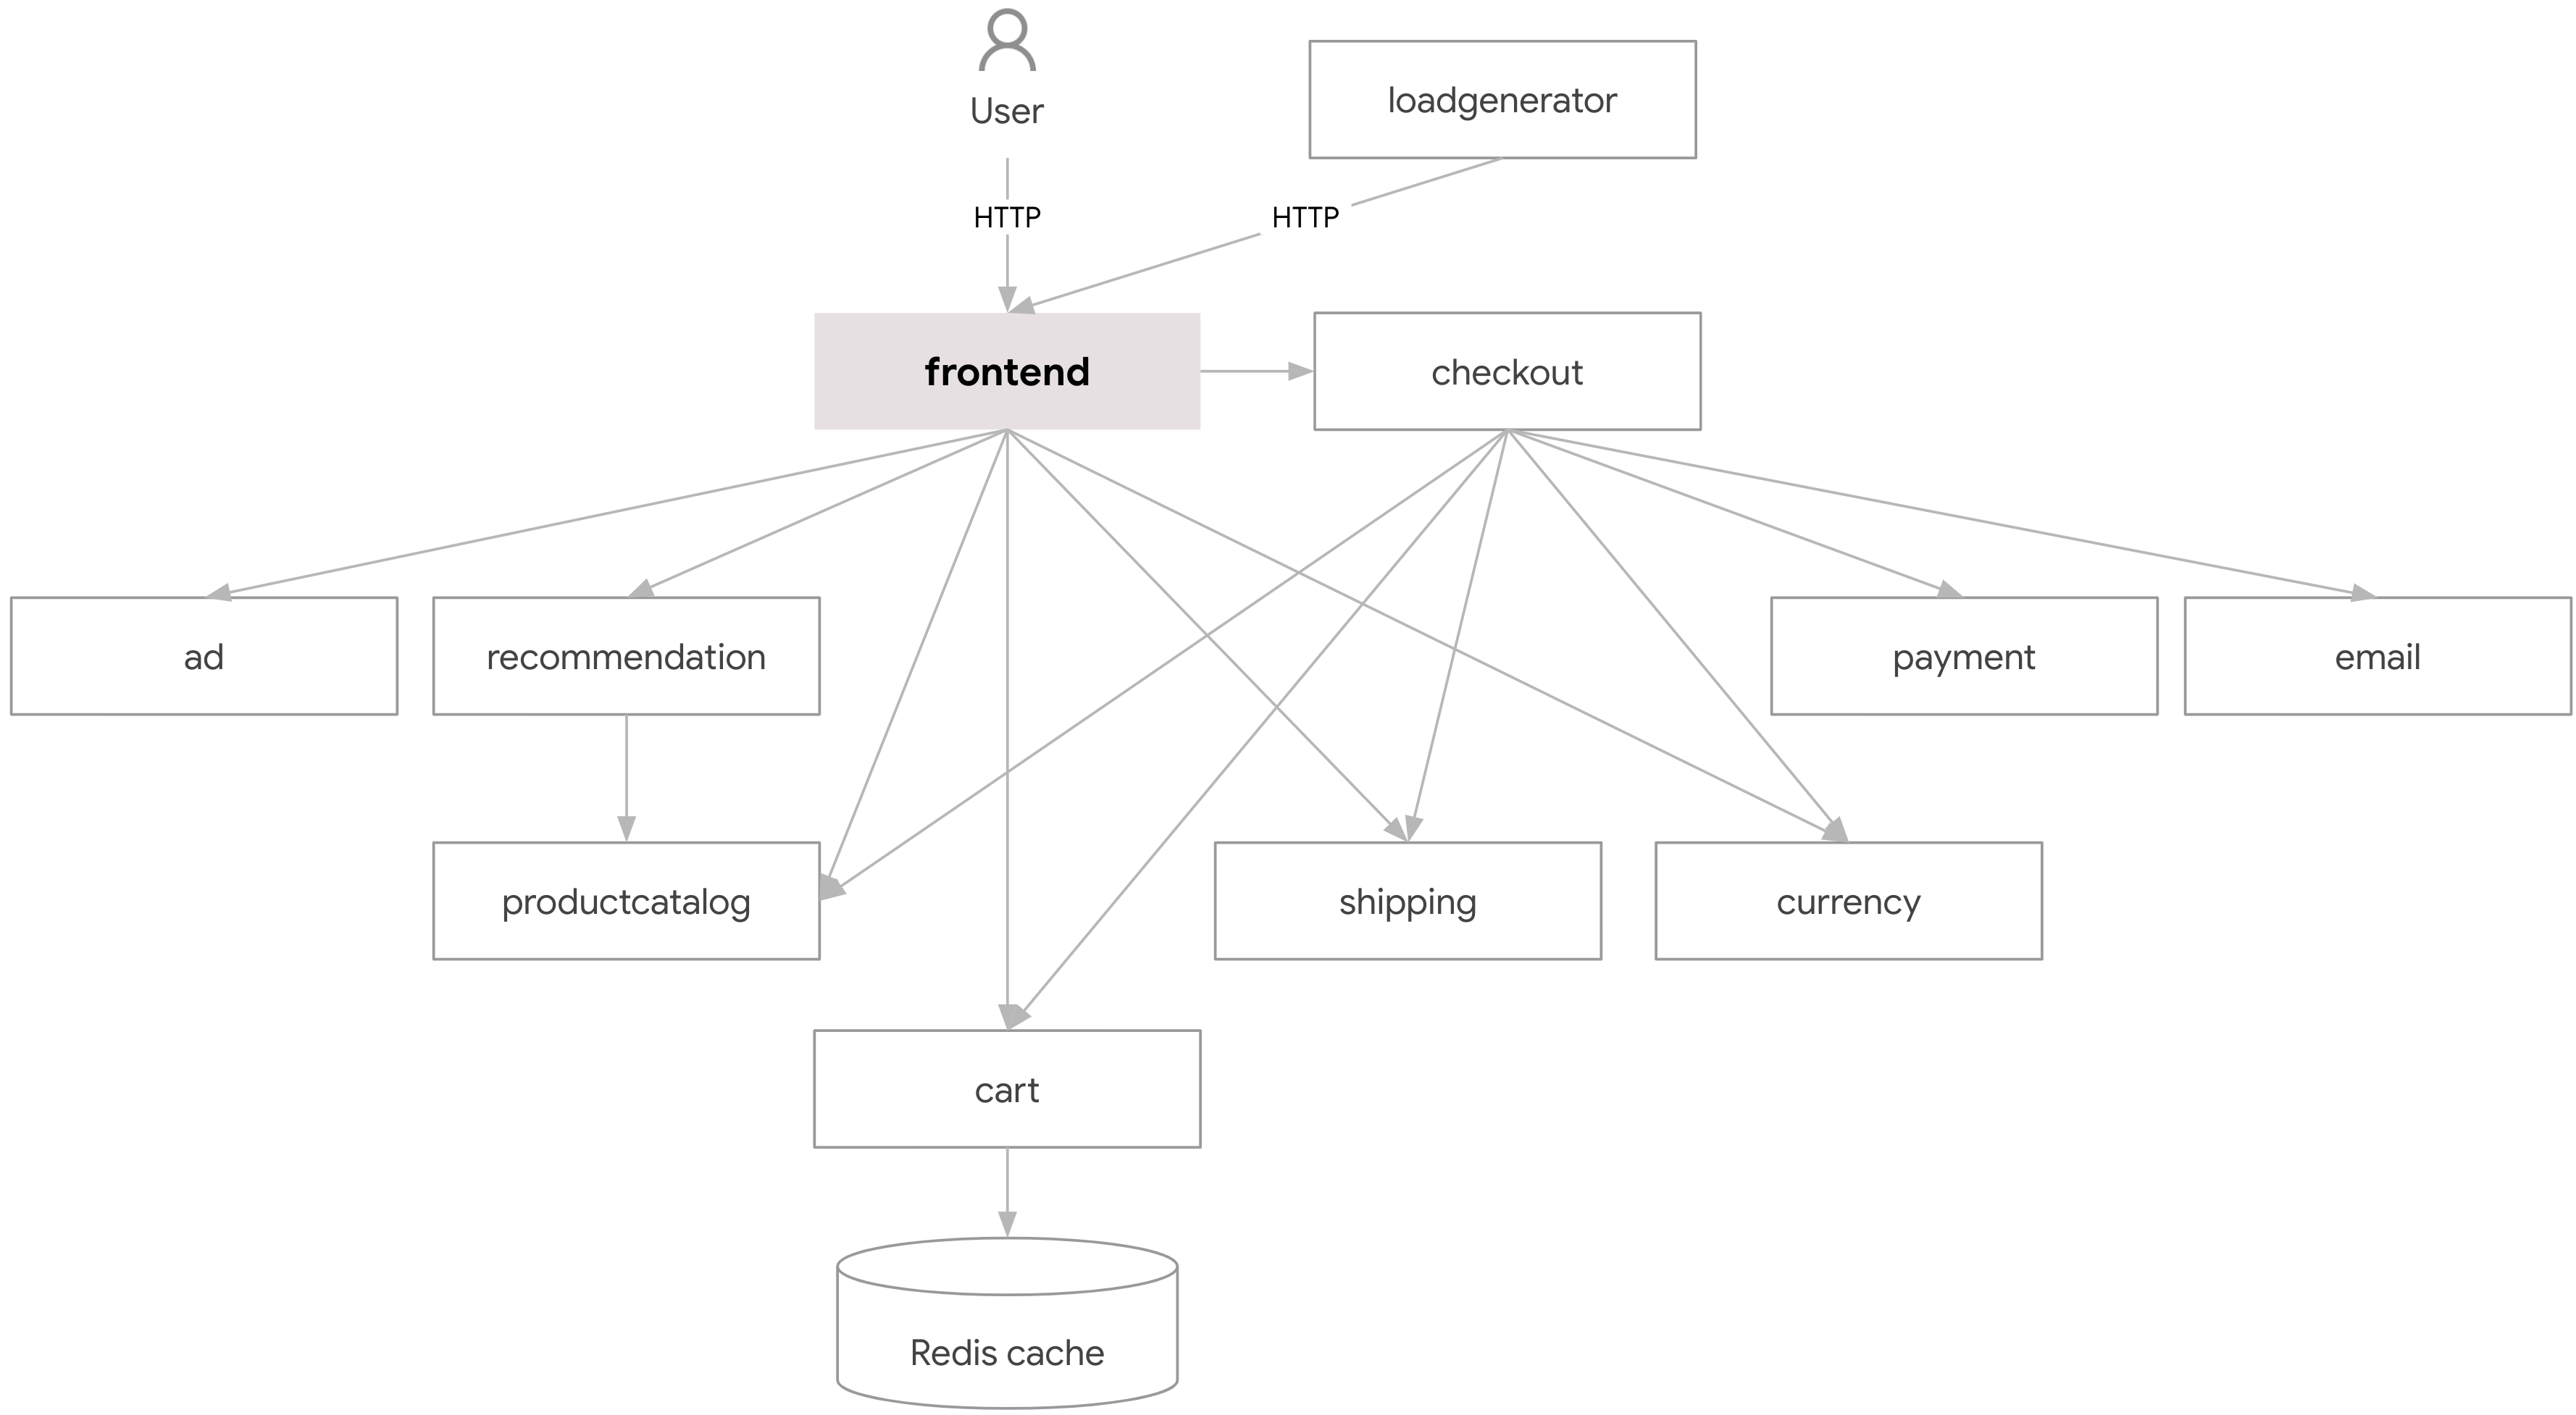
\includegraphics[width=0.9\textwidth]{figure/microservice/architecture-diagram.png}
	\caption{原始 Online Boutique 微服务架构}
	\label{fig:origin_microservice_arch}
\end{figure}

从架构上看，原系统服务拆分清晰，但商品库存没有被建模为独立状态。商品目录服务只负责展示商品基本信息，购物车服务只保存用户选择的商品和数量，二者之间没有库存约束。因此，本次开发没有在页面上简单写死库存数字，而是新增独立库存服务，使库存成为可以查询、扣减、恢复和监控的业务状态。

\subsection*{新增微服务设计}

本次开发新增了两个微服务：\texttt{inventoryservice} 和 \texttt{restockservice}。\texttt{inventoryservice} 是库存服务，负责维护每个商品的剩余库存、库存状态和仓库位置，并提供查询、预留、释放等能力；\texttt{restockservice} 是进货服务，作为管理员补货操作的后端入口，负责校验服务间调用凭证，并调用库存服务完成库存增加。扩展后的架构如图 \ref{fig:new_microservice_arch} 所示。

\begin{figure}[H]
	\centering
	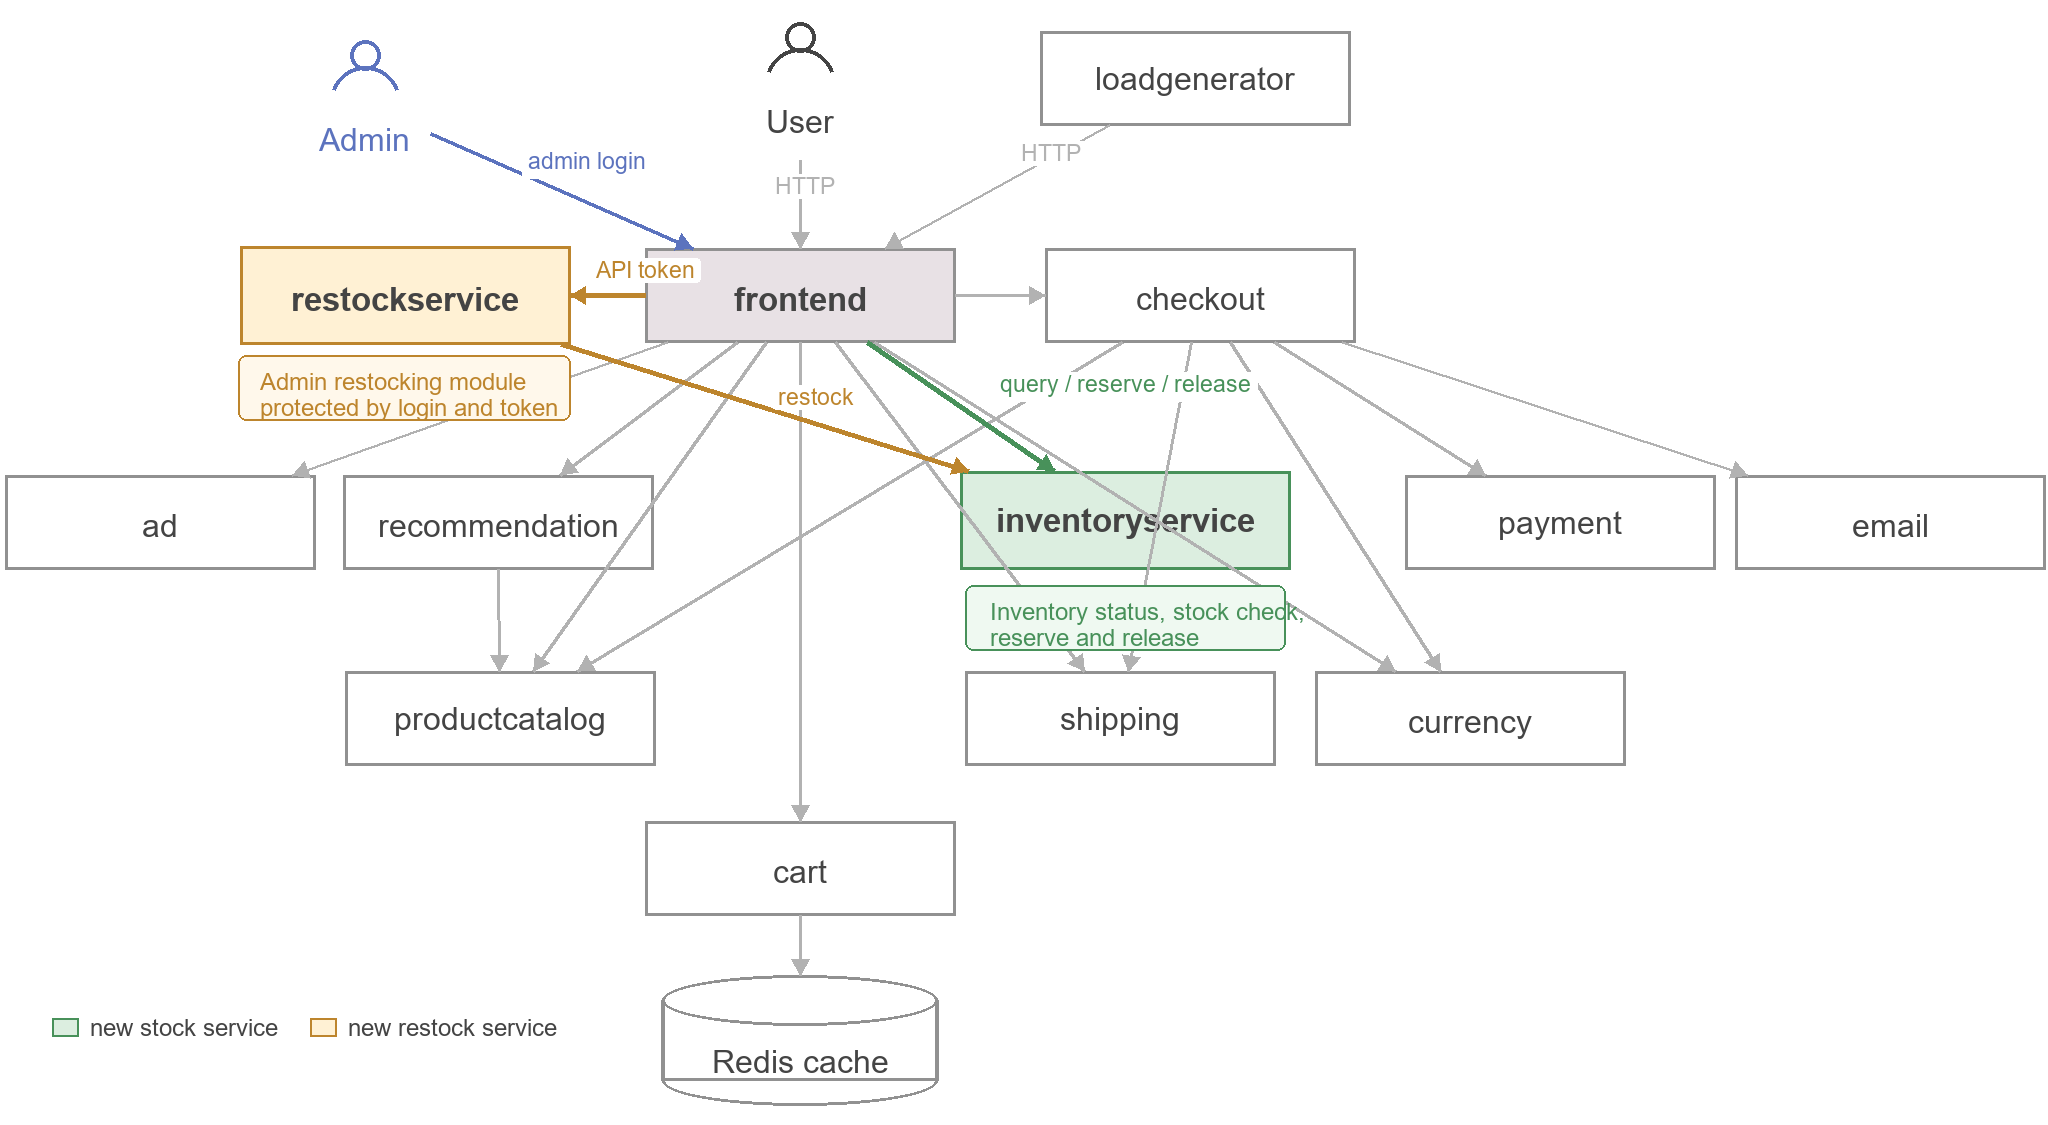
\includegraphics[width=0.9\textwidth]{figure/microservice/architecture-diagram-current.png}
	\caption{新增 inventoryservice 与 restockservice 后的系统结构}
	\label{fig:new_microservice_arch}
\end{figure}

扩展后系统形成了两条主要业务链路。第一条是普通用户购物链路：用户进入商品详情页时，\texttt{frontend} 调用 \texttt{inventoryservice} 查询当前库存，并在页面上展示剩余数量；用户加入购物车时，前端先请求库存服务预留库存，成功后再写入 \texttt{cartservice}；如果购物车写入失败，前端会调用库存服务释放刚才预留的库存，避免库存凭空减少；用户清空购物车时，系统也会把购物车中已有商品数量释放回库存。第二条是管理员进货链路：管理员访问独立的 \texttt{/admin/restock} 页面，登录成功后选择商品并输入进货数量，前端携带内部 API Token 调用 \texttt{restockservice}，再由进货服务调用库存服务增加库存。

\subsection*{库存服务实现概述}

\texttt{inventoryservice} 使用 Python 实现，核心职责是管理商品库存状态。服务启动时读取初始库存数据，并以商品 ID 为键保存库存数量、库存状态和仓库信息。库存状态根据剩余数量自动判断：库存为 0 时为缺货，库存较少时为低库存，其余情况为正常库存。这样前端不仅能显示“还剩多少件”，也能显示当前商品是否处于低库存或缺货状态。

库存服务提供三类核心接口。第一类是库存查询接口，用于商品详情页和管理员页面读取库存；第二类是库存预留接口，用于用户加入购物车时扣减库存；第三类是库存释放接口，用于购物车写入失败、清空购物车和管理员进货等场景。库存服务内部对库存变更操作加锁，避免并发请求同时修改同一份库存数据导致数量错误。服务还提供健康检查和 metrics 指标，便于 Kubernetes 探针和后续监控系统判断服务状态。

这种设计的关键点在于：库存判断被放在服务端，而不是只依赖前端页面限制。即使用户绕过页面直接构造请求，也必须经过库存服务校验，无法购买超过库存的数量。这样可以让库存约束成为系统后端的一部分，而不是单纯的页面展示逻辑。

\subsection*{进货服务实现概述}

\texttt{restockservice} 同样使用 Python 实现，它不直接保存库存，而是承担管理员进货入口的角色。这样拆分的原因是普通用户购买商品和管理员补充库存属于不同业务角色，如果把进货逻辑混在商品详情页或购物车逻辑中，会让用户流程和管理流程混杂在一起，也不利于后续权限控制、进货记录、供应商管理等功能扩展。

进货流程采用两层保护。第一层是前端管理员登录，管理员需要使用账号密码进入 \texttt{/admin/restock} 页面；第二层是服务间 API Token，只有携带正确 Token 的前端请求才能调用进货服务。这样的设计区分了“浏览器访问权限”和“服务间调用权限”：前者保护管理员页面，后者保护进货接口本身。

当管理员提交进货数量后，\texttt{frontend} 会向 \texttt{restockservice} 发送请求；进货服务校验 Token 和参数后，再调用 \texttt{inventoryservice} 更新库存。操作成功后，页面显示进货成功弹窗，管理员点击确认后刷新页面，从而看到更新后的库存数量。相关界面和操作效果截图放在附录 \ref{sec:appendix_microservice_figures} 中。

\subsection*{前端集成改造}

原 \texttt{frontend} 服务使用 Go 实现，是用户访问系统的统一入口。本次开发在前端中增加了库存查询、库存预留、库存释放和管理员进货页面的调用逻辑。普通用户打开商品详情页时，页面会展示该商品的剩余库存、库存状态和仓库位置；商品数量选择框会根据库存动态限制最大可选数量，避免页面上直接选择超过库存的数量。

加入购物车时，前端不再直接写入购物车，而是先向库存服务申请预留库存。只有库存预留成功后，才继续调用购物车服务。如果购物车服务写入失败，前端会立即释放库存，完成一次简单的补偿操作。清空购物车时，前端先读取购物车内容，再调用购物车服务清空，最后把购物车中原有商品数量逐项释放回库存。通过这些改造，系统实现了“加入购物车扣减库存、清空购物车恢复库存、库存不足拒绝加入”的基本闭环。

管理员页面则被设计为独立模块，而不是放在普通商品购买流程中。管理员访问 \texttt{/admin/restock} 后先看到登录页面，登录成功后进入进货页面。页面列出商品、当前库存和进货输入框，管理员提交后由前端调用进货服务。这样既保持了普通用户页面的简洁，也让管理操作有清晰的入口和权限边界。

\subsection*{部署与测试}

两个新增服务都补充了 Dockerfile、Kubernetes Deployment 和 Service 配置，并加入到 skaffold 构建流程中。\texttt{frontend} 通过环境变量读取库存服务和进货服务地址，例如 \texttt{INVENTORY\_SERVICE\_URL} 和 \texttt{RESTOCK\_SERVICE\_URL}。在 Kubernetes 中，服务之间不使用 \texttt{localhost} 通信，而是通过 Service 名称进行访问，例如 \texttt{inventoryservice} 和 \texttt{restockservice}。这样可以适应 Pod 动态创建和销毁的环境。

测试方面，库存服务重点验证库存查询、库存预留、库存不足拒绝、库存释放和异常商品 ID 等场景；进货服务重点验证 Token 校验、参数校验、进货成功和依赖库存服务失败等场景。前端功能则通过手动操作验证：商品详情页能看到库存，加入购物车后库存减少，清空购物车后库存回滚，管理员登录后可以进货，进货成功后弹窗提示并刷新页面。测试截图和 Kubernetes 运行状态截图统一放在附录中。

\subsection*{本部分小结}

本部分在 Online Boutique 原有系统基础上新增了库存服务和进货服务，并完成了前端集成、容器化部署和功能测试。库存服务让商品库存从静态页面信息变成独立业务状态，支持查询、扣减、释放和监控；进货服务将管理员补货从普通购买流程中拆分出来，并通过管理员登录和 API Token 进行保护。经过改造后，系统形成了较完整的库存业务闭环：用户购买会占用库存，取消购物车会恢复库存，库存不足会拒绝请求，管理员可以在独立页面补充库存。该过程体现了微服务系统中服务拆分、接口协作、状态一致性、服务发现和可测试性的基本思想。


\section{部署 故障注入与监控 数据采集分析}
该实验所使用的环境、工具 ...

\section{fluxev论文复现}


\section{项目测试}
\subsection*{Selenium IDE测试}

我们使用Selenium IDE进行系统功能自动化测试，通过录制前端操作打通微服务从浏览商品，到选购，到广告，到下单的全流程，实现了系统功能的自动化测试，全程测试约10s，下附一张测试通过的图片\ref{fig:selenium}，相关的测试脚本文件可以在我们仓库的test文件夹下的selenium文件夹下找到

\begin{figure}[htbp]
	\centering
	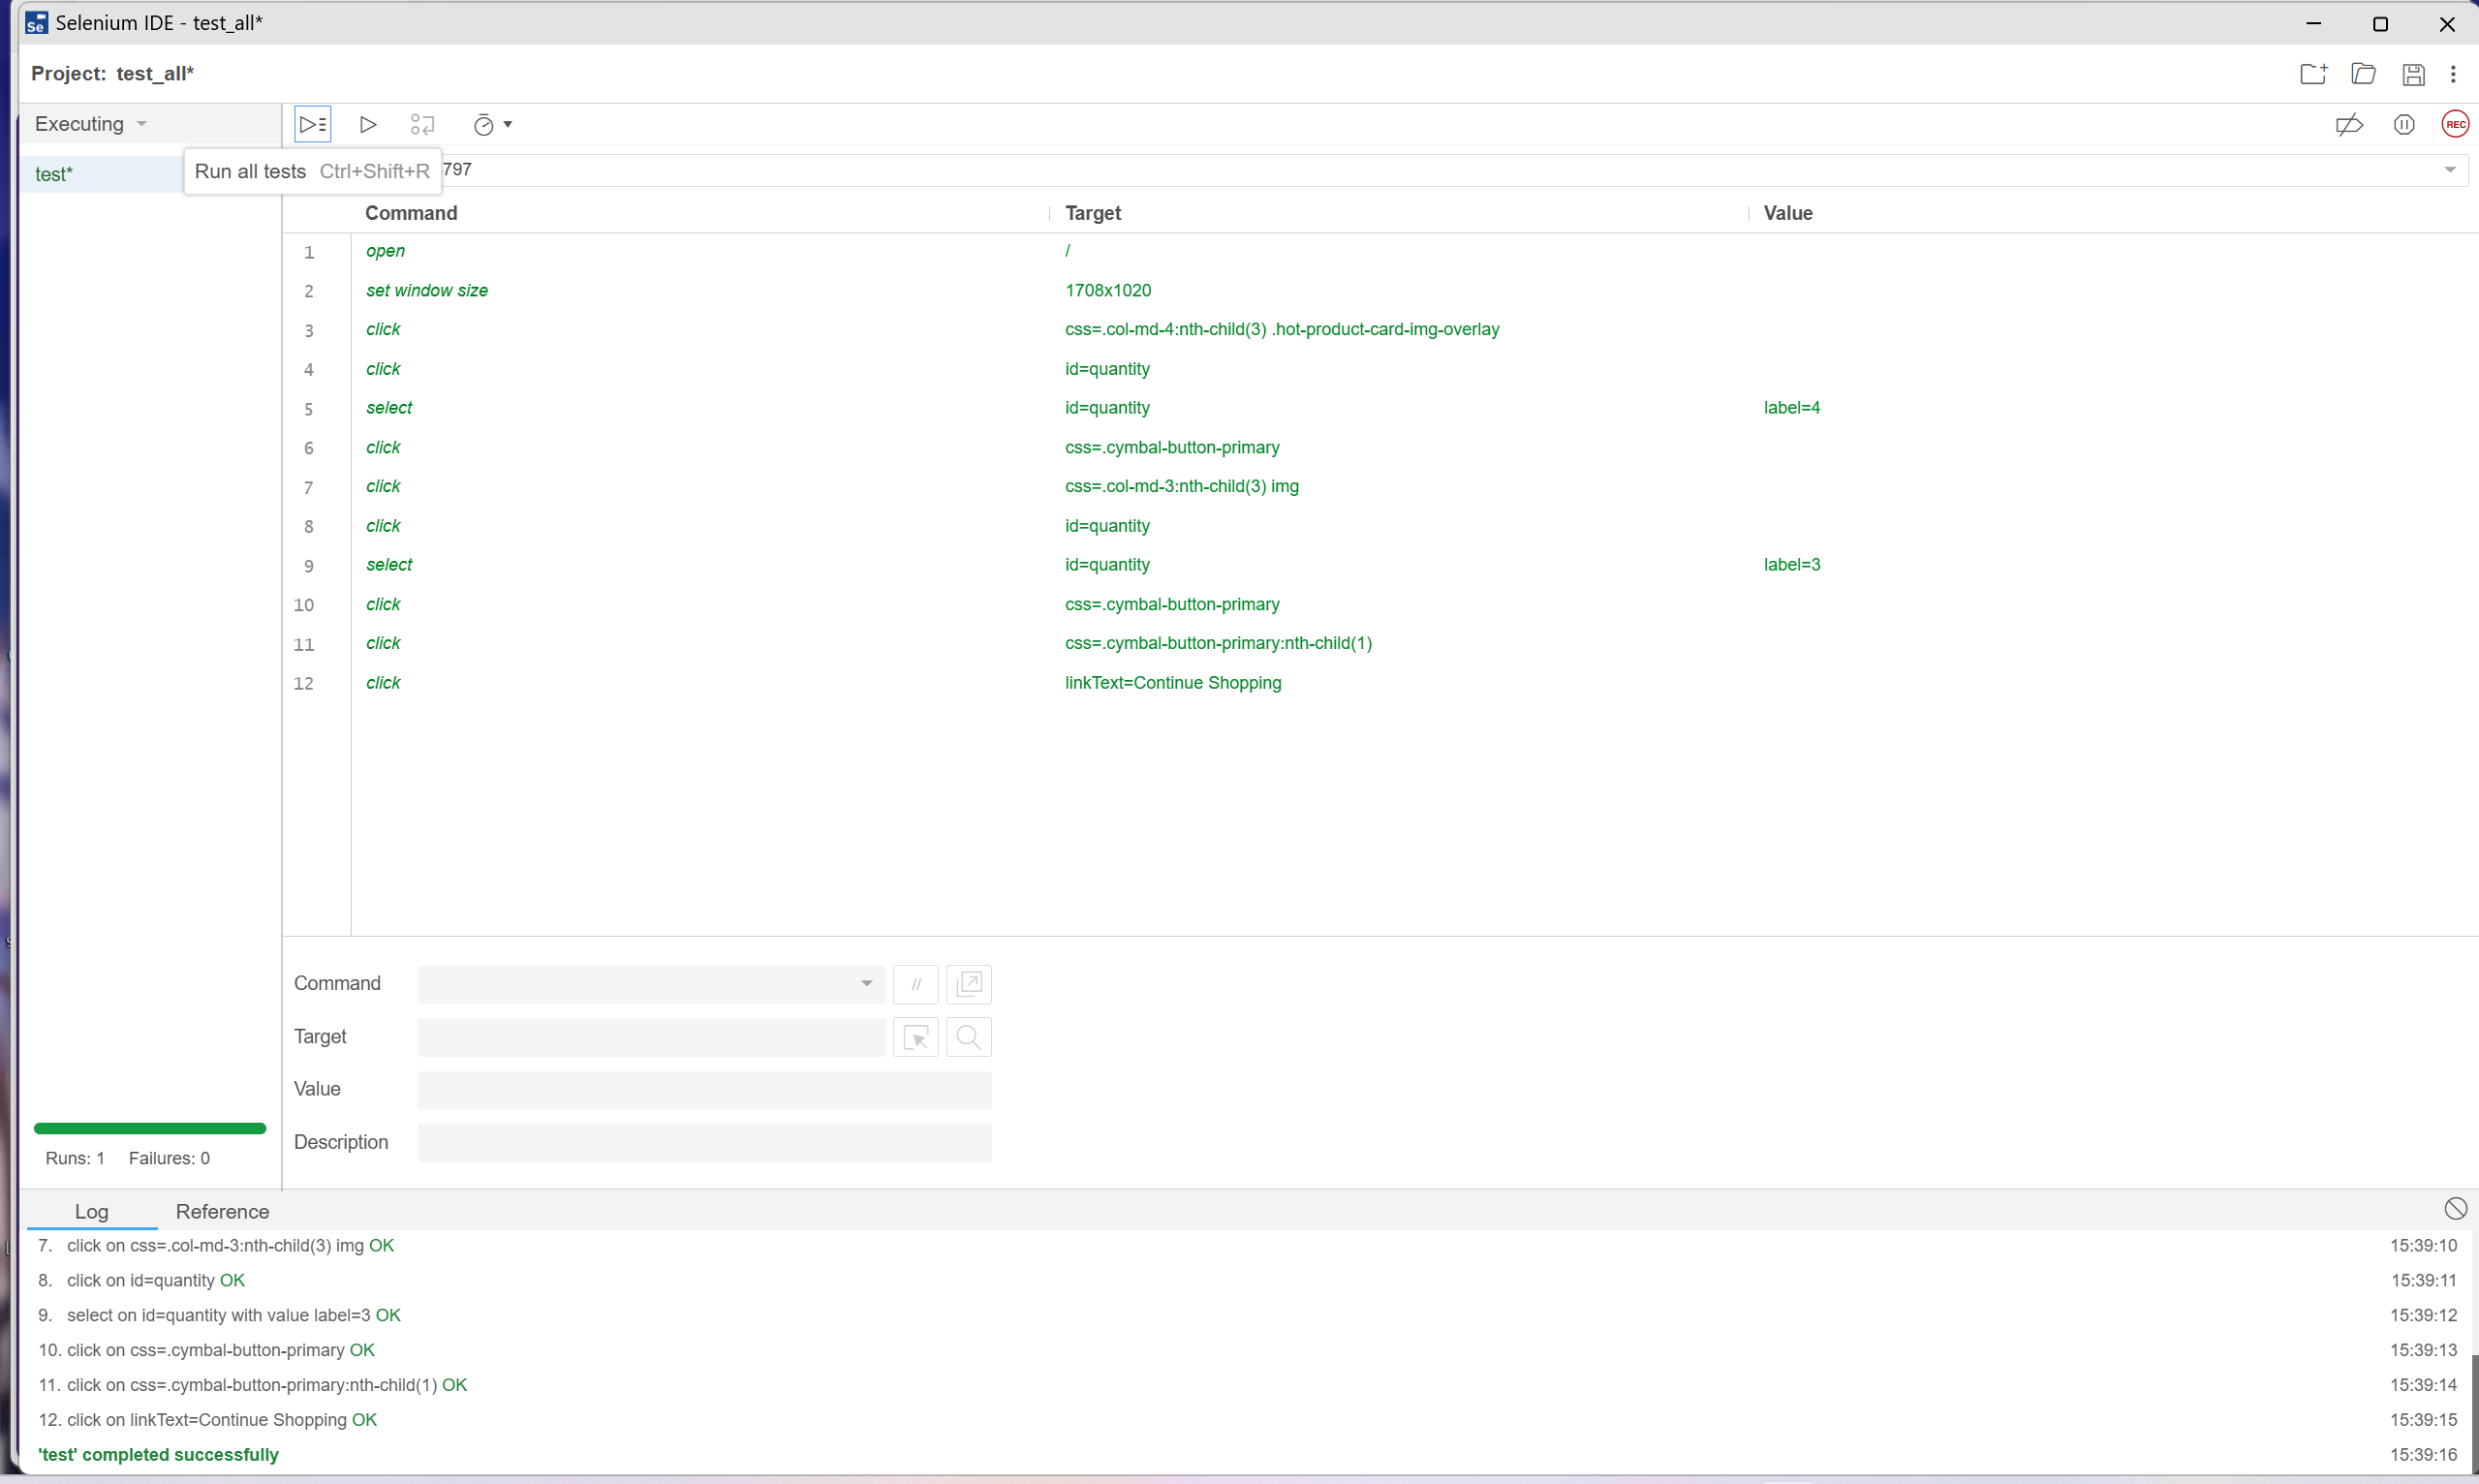
\includegraphics[width=0.8\textwidth]{./figure/test/selenium.png}
	\caption{selenium ide自动化测试}
	\label{fig:selenium}
\end{figure}
\subsection*{Jmeter自动化测试}




\section{LightLog复现及其消融与对比实验}
\subsection*{数据集构建}
\subsubsection{日志采集}

为了构造我们自己的log数据集，我们使用了fluent来进行日志的采集工作，通过修改fluent-configmap文件完成将采集的日志存储到本地文件中的任务，但fluent是以pod的形式存在于k8s集群中的，所以我们需要在minikube启动的时候进行数据卷挂载，将fluent记录日志的目录挂载到宿主机中。至此我们解决了日志收集的存储问题

我们通过jmeter持续对微服务发起请求，在进行上述jmeter自动化测试的时候我们便已收集了许多日志，但这仍然不足以构建出一个数据集，于是我们编写一个持续性请求的测试脚本不断进行请求，并结合下一节的内容构建数据集

\subsubsection{chaosmesh故障注入}

使用jmeter自动化请求可以收集到大量的正常日志，但异常日志并不那么容易产生，为了人为制造异常日志，我们使用chaosmesh故障注入，实验时间设为一小时。我们设计了如表\ref{tab:chaos-core}中所示的三种chaosmesh故障，使用单个注入或者组合注入的方式进行注入并采集到符合要求的异常日志

这里使用网络混沌实验来模拟真实场景中大部分的网络波动场景，这些混沌实验可以作用于grpc协议包，使其不仅可以模拟用户与服务器之间的网络波动，还能模拟微服务之间互相请求的波动。我们调高了混沌实验的相关性参数，使得异常发生得“有迹可循”，尽量模拟真实场景的日志情况，也为后续复现各种处理序列型数据的模型结构提供了方便。

\begin{table}[htbp]
	\centering
	\caption{Chaos Mesh 网络混沌实验核心参数对比}
	\label{tab:chaos-core}
	\begin{tabular}{|l|l|l|l|}
		\hline
		\textbf{参数} & \textbf{test-lost} & \textbf{test-corrupt} & \textbf{test-delay} \\ \hline
		动作 (action) & loss & corrupt & delay \\ \hline
		持续时间 & 1h & 1h & 1h \\ \hline
		方向 & to & to & to \\ \hline
		主要参数 & loss=30\% & corrupt=25\% & latency=2s \\ \hline
		抖动 (jitter) & - & - & 3s \\ \hline
		相关性 (correlation) & 90\% & 90\% & 90\% \\ \hline
		目标 Pod 数量 & 10 & 10 & 10 \\ \hline
	\end{tabular}
\end{table}

\subsection*{构建数据集}

我们编写脚本，通过识别日志中的关键词（如error，fail等），网络状态码（如400，500等），响应时间（过长的响应时间等异常情况）等异常因素综合判定日志是否为异常日志进行数据标注。有关数据集处理的代码可以在我们仓库的lightlog目录下的dataset目录下找到。

我们借鉴LightLog中\cite{wang2022lightlog}的有关数据集处理，由于我们收集的日志没有记录块id，所以我们使用了BGL数据集的滑动窗口机制构建自己的数据集，鉴于我们的数据集是个人电脑收集的，数量并不如超级计算机直接生成的一般大。所以使用了相比论文中提到的BGL数据集300条日志为一条序列更短的序列长度：20。使用8000条正常序列与8000条异常序列构造出训练数据集，将剩余采集到的正常序列与相当其2.9\%的异常序列混合作测试数据集。训练集中正常序列与异常序列1：1的比例是为了让模型在训练的时候可以充分提取正常序列和异常序列的特征，而测试集中的比例是为了保证在模型测试的时候可以得到对标真实情况的测试，使其可以应用于真实场景。我们使用了论文中提到的hdfs数据集中正常与异常数据的比例，最终构建了约23w条序列作为测试集。

\subsection*{LightLog复现}

\subsection*{LightLog消融实验}

\subsection*{LogAnomaly与LogRobust的复现及对比实验}

\subsubsection{LogAnomaly复现}

\subsubsection{LogRobust复现}

我们阅读了LogRobust\cite{zhang2019robust}并对其进行了复现，下面介绍LogRobust论文中提到的模型原理

\begin{figure}[htbp]
	\centering
	\begin{subfigure}{0.45\textwidth}
		\centering
		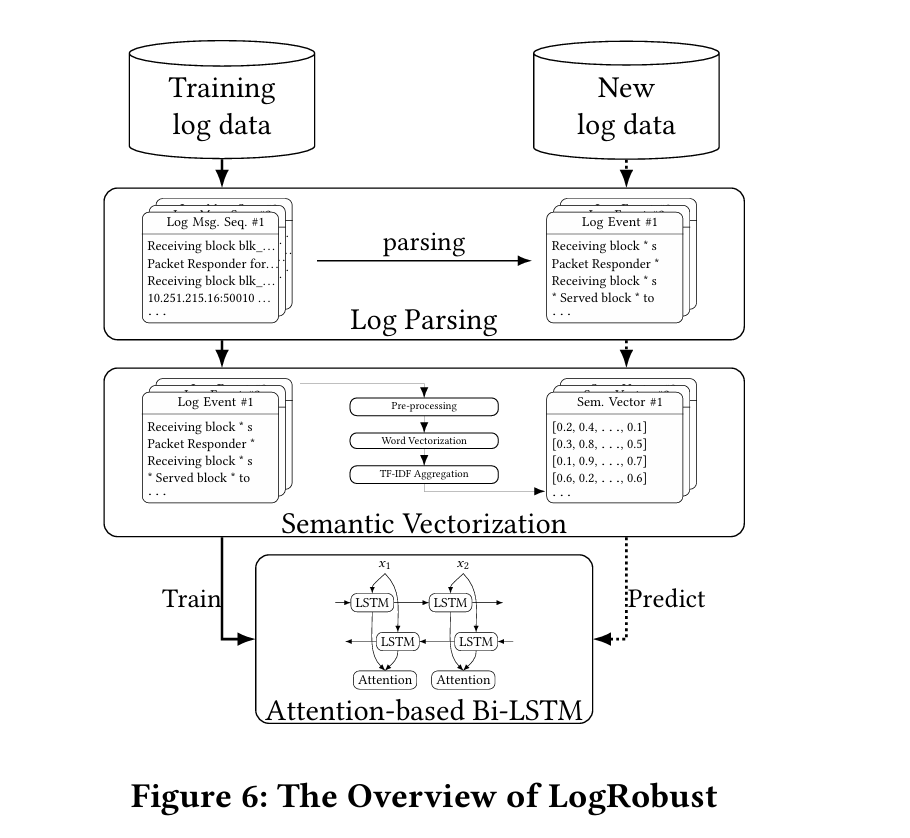
\includegraphics[width=\textwidth]{./figure/LightLog/LogRobust/data_process_robust.png}
		\caption{数据预处理}
		\label{fig:dataprocess}
	\end{subfigure}
	\hfill
	\begin{subfigure}{0.45\textwidth}
		\centering
		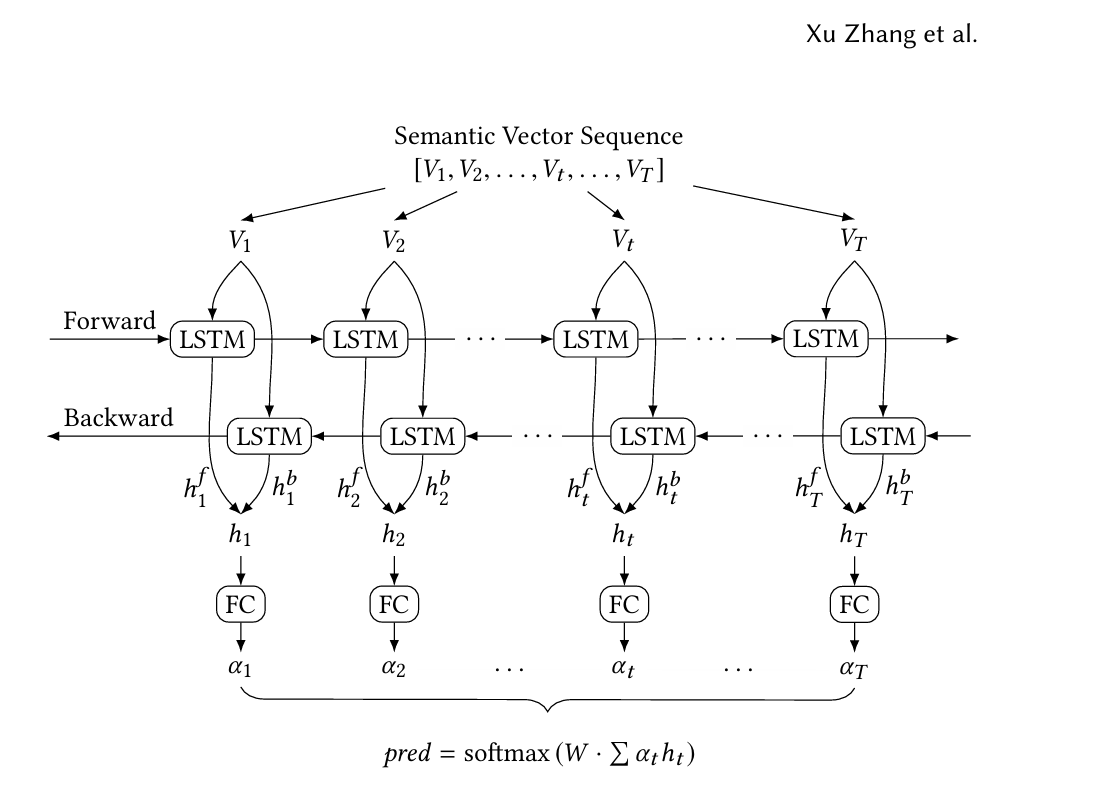
\includegraphics[width=\textwidth]{./figure/LightLog/LogRobust/model_robust.png}
		\caption{模型架构}
		\label{fig:model}
	\end{subfigure}
	\caption{LogRobust方法}
	\label{fig:LogRobust}
\end{figure}

图\ref{fig:LogRobust}中展示了LogRobust使用的方法，图片来自于LogRobust论文\cite{zhang2019robust}。

如图\ref{fig:dataprocess}所示，LogRobust先对日志序列进行预处理，Log Seq（日志序列）会被转化为Log Event（结构化日志事件），在这之后结构化日志事件会被预训练的300维fasttext向量编码为语义向量，送入模型中。

如图\ref{fig:model},语义向量将被送入如图的模型架构中，日志事件会按时序送入一个双向LSTM网络架构中，双向的LSTM可以保证该架构具有日志序列的全局信息，为下面的注意力机制提供更全面的信息。

网络使用加性注意力，对每个时间步进行注意力输出，该注意力层在双层LSTM后。该层会给每个日志事件进行打分，评判出日志事件的重要性。再之后经过一个全连接层与softmax层输出两个值，正常概率和异常概率，用此综合评判一条日志序列是否异常。

在附录中我们提供了LogRobust的训练曲线作为参考\ref{fig:LogRobustTrain}。有关LogRobust复现的代码存放在项目仓库中LightLog下的LogRobust文件夹下


\subsubsection{对比实验结果及分析}

\section{智能体运维}
通过这次实验记录自己在本次实验中所遇到的问题，以及心得感悟即相关问题和解决方法。如果遇到异常情况，或者无法完成任务时，也请分析错误产生的原因。

\section{总结与展望}

\begin{thebibliography}{99}

\bibitem{wang2022lightlog}
Zumin Wang, Jiyu Tian, Hui Fang, Liming Chen, and Jing Qin.
\newblock LightLog: A lightweight temporal convolutional network for log anomaly detection on the edge.
\newblock \emph{Computer Networks}, 203:108616, 2022.

\bibitem{zhang2019robust}
Xu Zhang, Yong Xu, Qingwei Lin, Bo Qiao, Hongyu Zhang, Yingnong Dang, Chunyu Xie, Xinsheng Yang, Qian Cheng, Ze Li, Junjie Chen, Xiaoting He, Randolph Yao, Jian-Guang Lou, Murali Chintalapati, Furao Shen, and Dongmei Zhang.
\newblock Robust log-based anomaly detection on unstable log data.
\newblock In \emph{Proceedings of the 2019 27th ACM Joint Meeting on European Software Engineering Conference and Symposium on the Foundations of Software Engineering (ESEC/FSE 2019)}, pages 807--817, 2019.

\bibitem{meng2019loganomaly}
Weibin Meng, Ying Liu, Yichen Zhu, Shenglin Zhang, Dan Pei, Yuqing Liu, Yihao Chen, Ruizhi Zhang, Shimin Tao, Pei Sun, et al.
\newblock Loganomaly: Unsupervised detection of sequential and quantitative anomalies in unstructured logs.
\newblock In \emph{IJCAI}, volume 19, pages 4739--4745, 2019.

\bibitem{li2021fluxev}
Jia Li, Shimin Di, Yanyan Shen, and Lei Chen.
\newblock FluxEV: A fast and effective unsupervised framework for time-series anomaly detection.
\newblock In \emph{Proceedings of the 14th ACM International Conference on Web Search and Data Mining (WSDM '21)}, pages 824--832, 2021.

\end{thebibliography}
\section{附录}
\subsection*{新增微服务相关截图}
\label{sec:appendix_microservice_figures}

\begin{figure}[htbp]
	\centering
	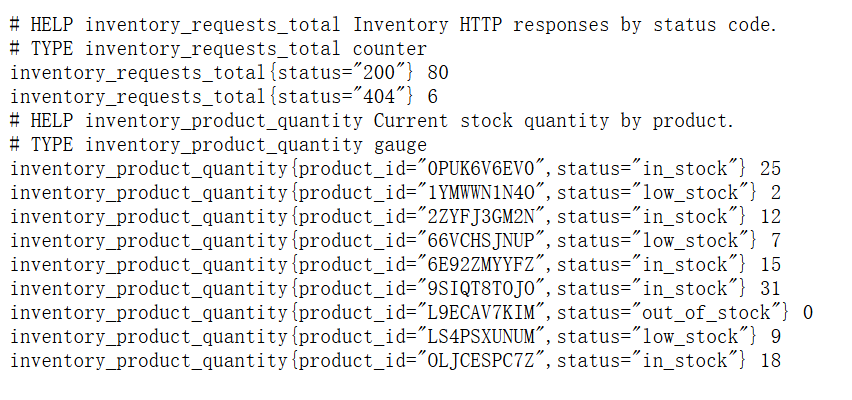
\includegraphics[width=0.85\textwidth]{figure/microservice/service_metrics.png}
	\caption{inventoryservice 监控指标截图}
	\label{fig:appendix_service_metrics}
\end{figure}

\begin{figure}[htbp]
	\centering
	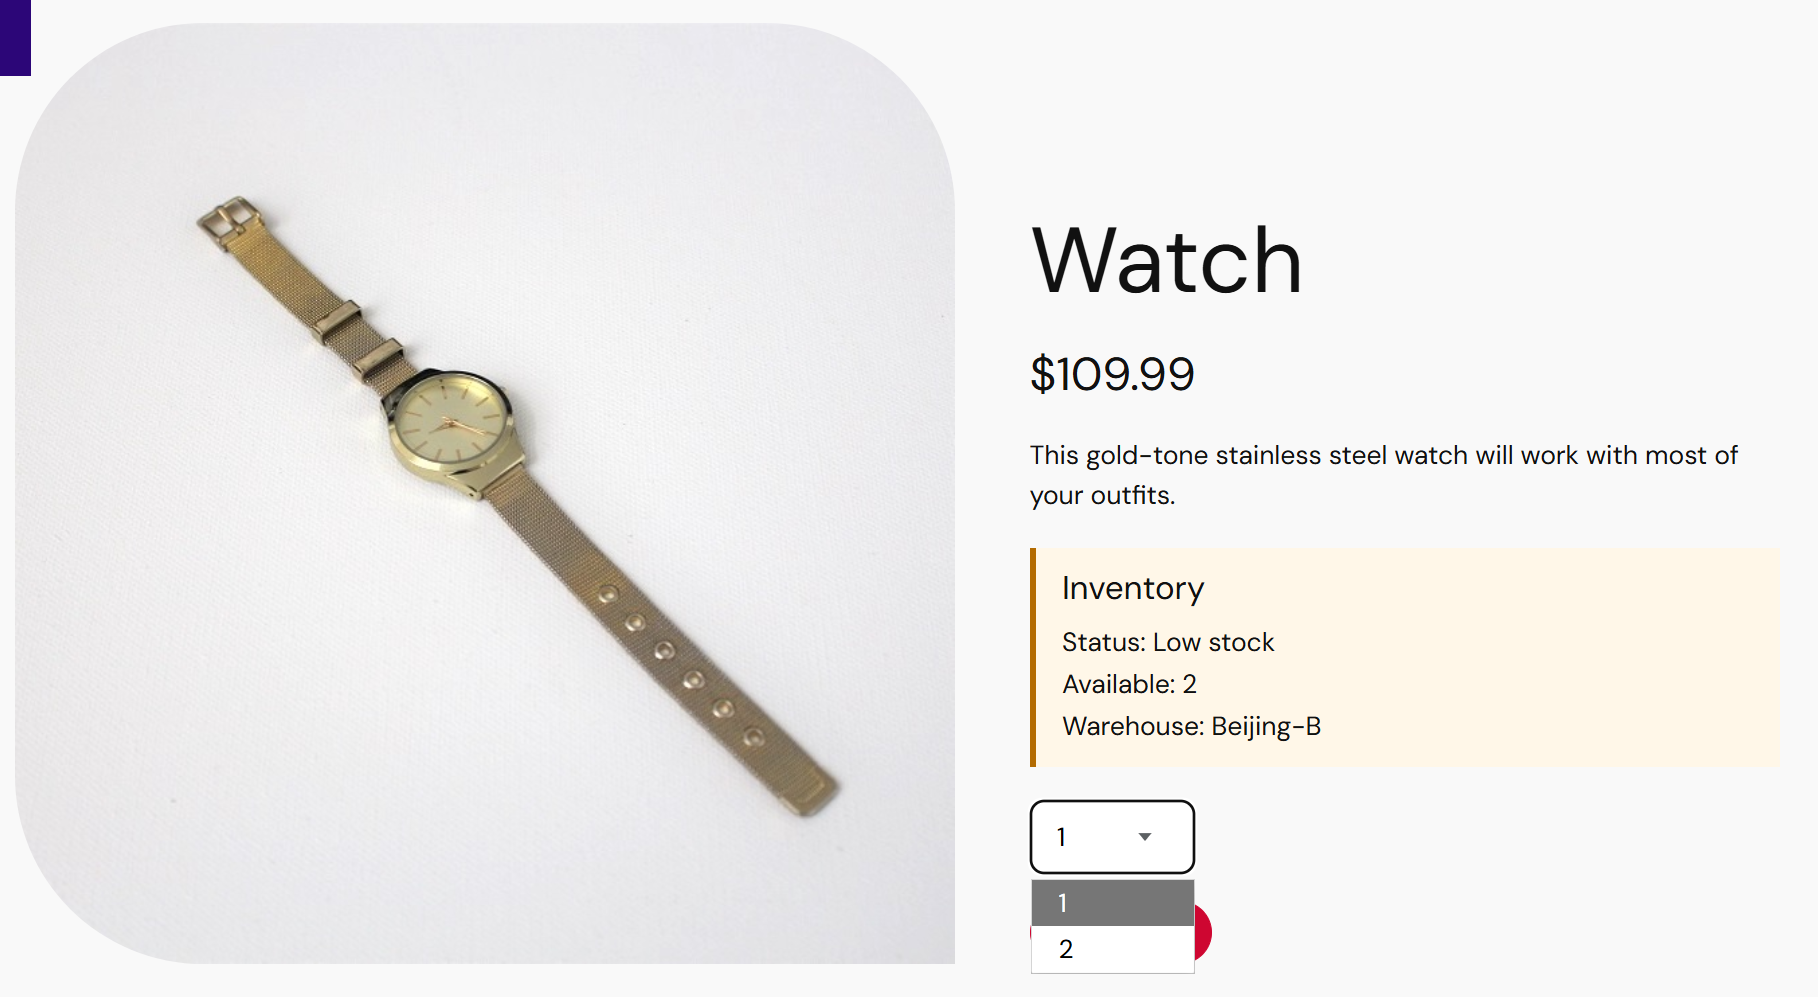
\includegraphics[width=0.85\textwidth]{figure/microservice/watch.png}
	\caption{商品详情页库存展示截图}
	\label{fig:appendix_inventory_watch}
\end{figure}

\begin{figure}[htbp]
	\centering
	\begin{minipage}{0.45\textwidth}
		\centering
		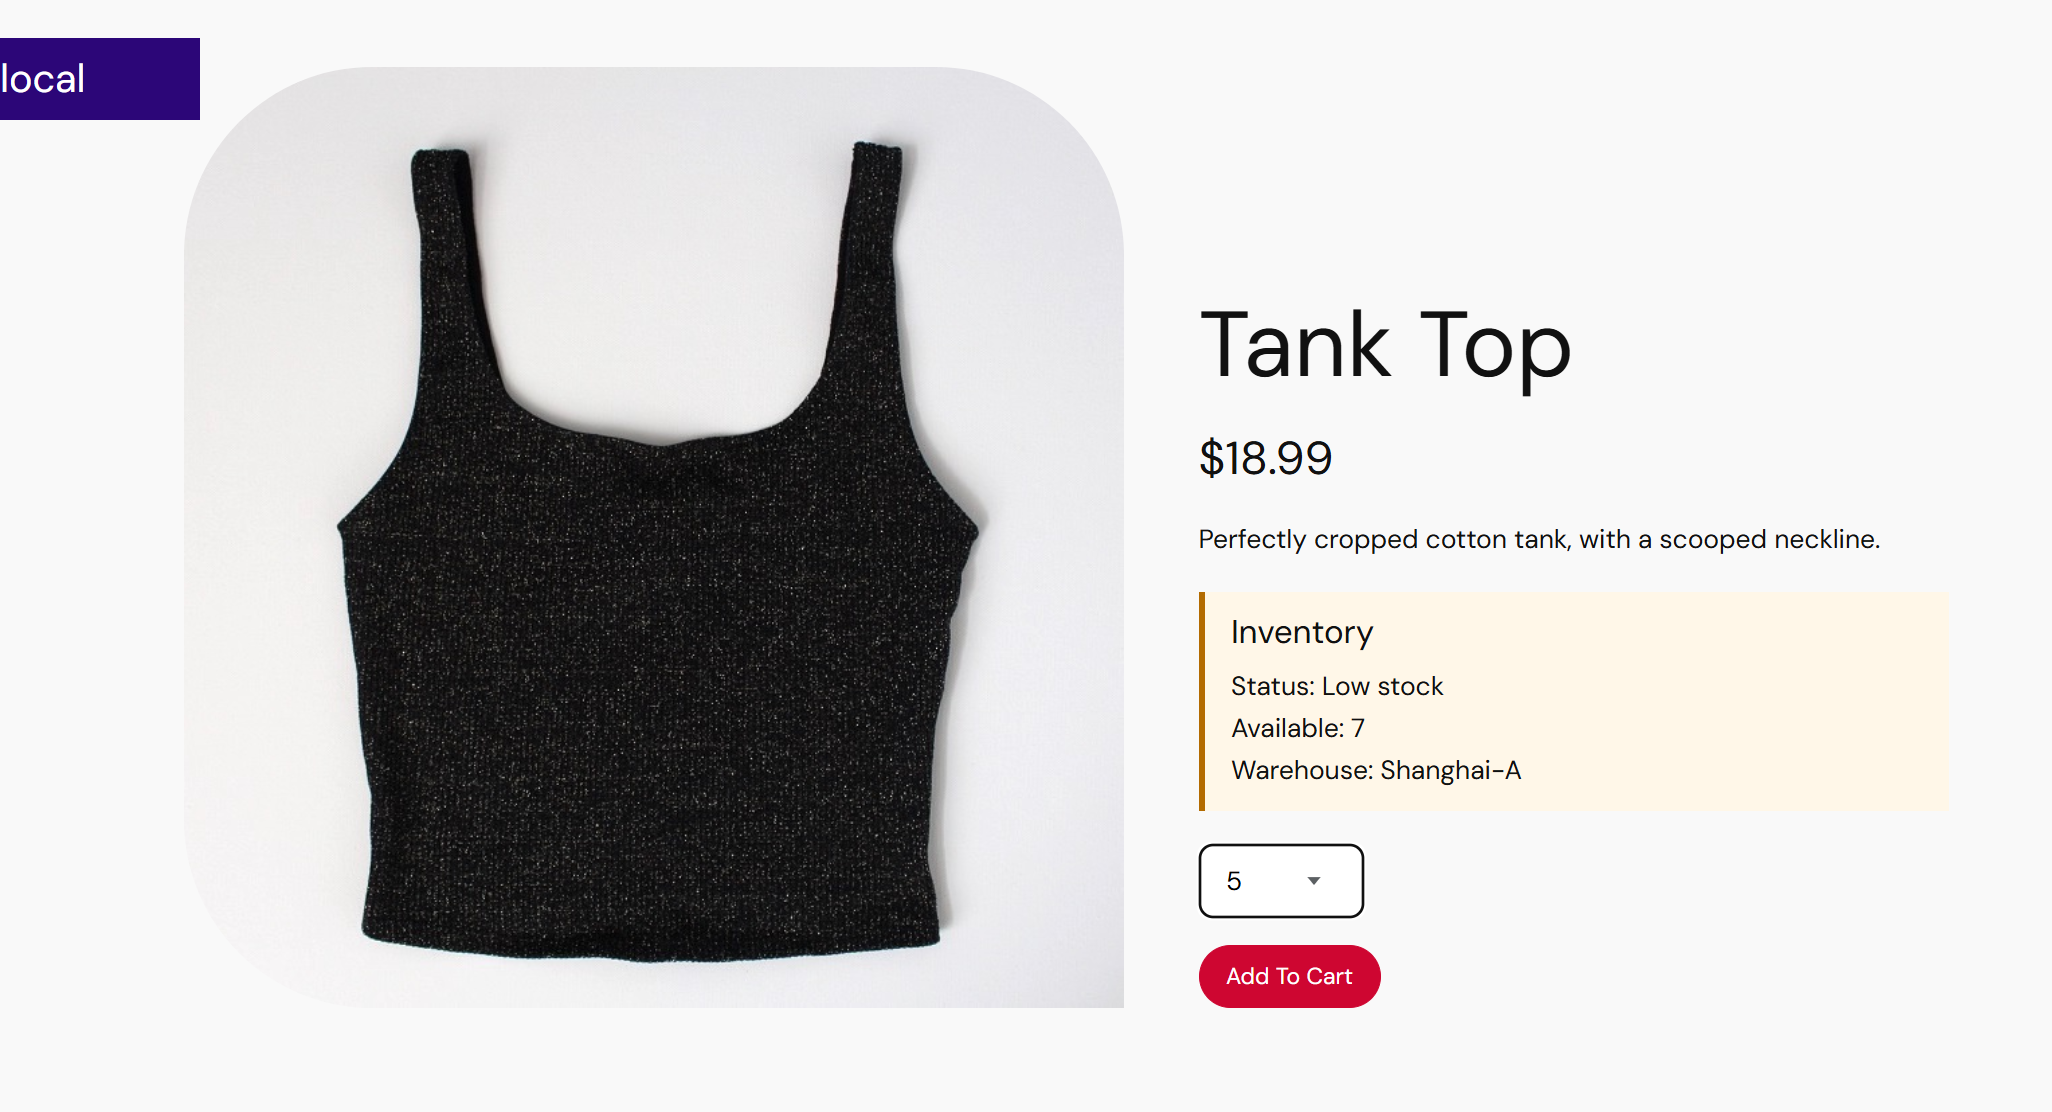
\includegraphics[width=\textwidth]{figure/microservice/beforeenter.png}
		加入购物车前
	\end{minipage}
	\hfill
	\begin{minipage}{0.45\textwidth}
		\centering
		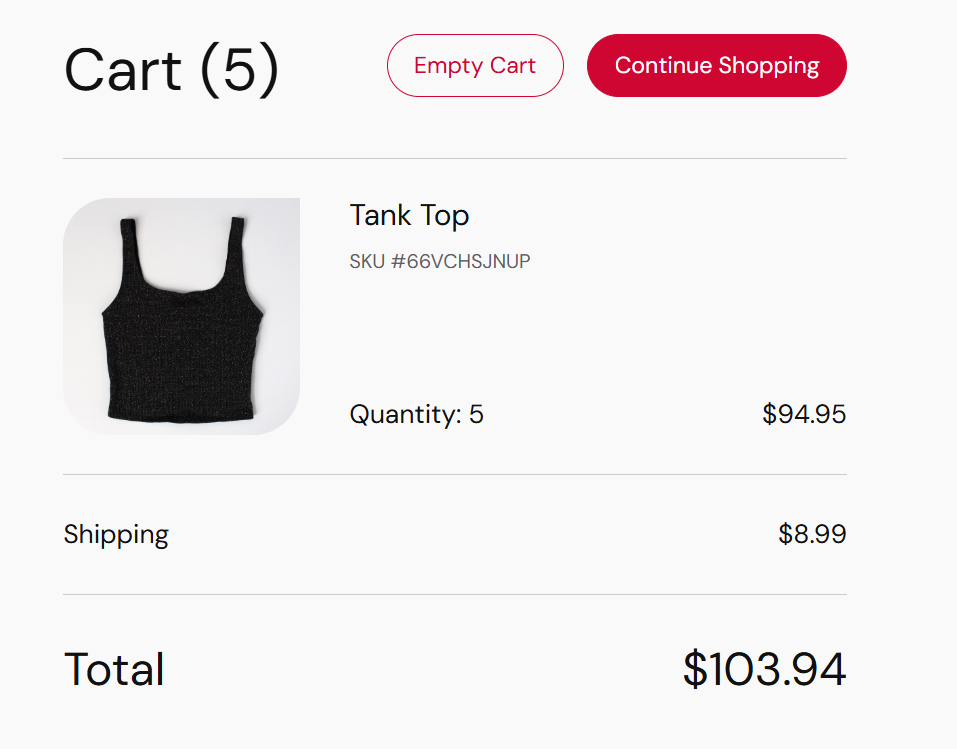
\includegraphics[width=\textwidth]{figure/microservice/buyit.png}
		选择购买数量
	\end{minipage}
	\caption{库存扣减前的商品状态}
	\label{fig:appendix_inventory_before}
\end{figure}

\begin{figure}[htbp]
	\centering
	\begin{minipage}{0.45\textwidth}
		\centering
		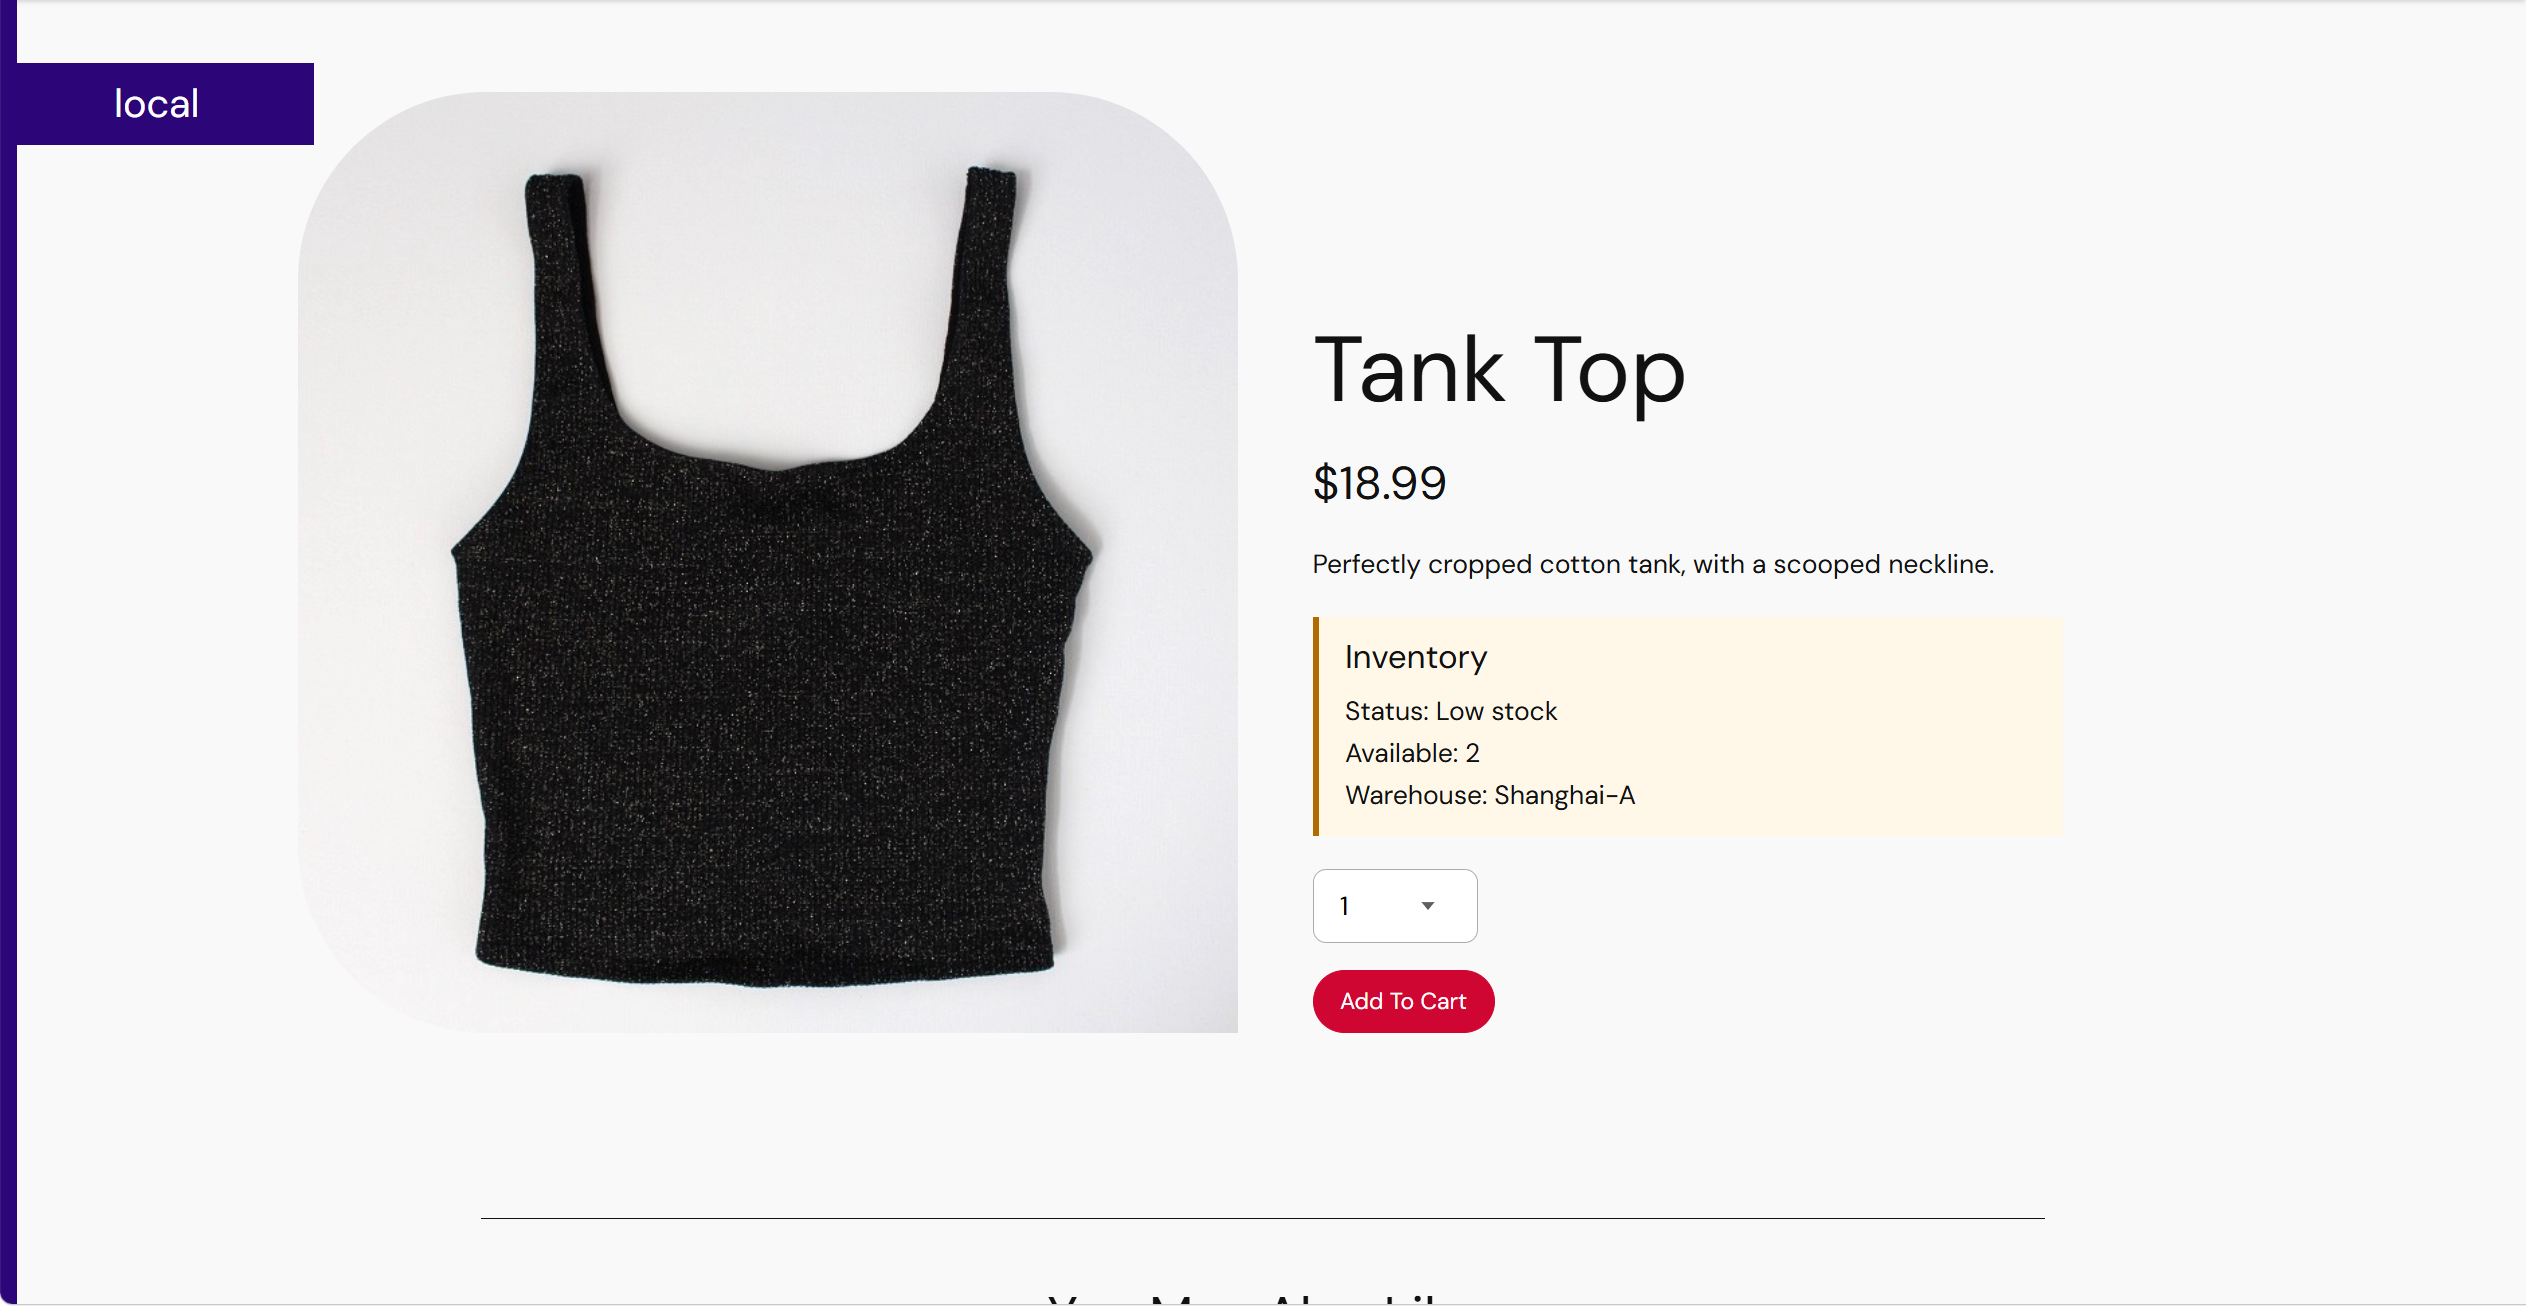
\includegraphics[width=\textwidth]{figure/microservice/afterjoinit.png}
		加入购物车后库存减少
	\end{minipage}
	\hfill
	\begin{minipage}{0.45\textwidth}
		\centering
		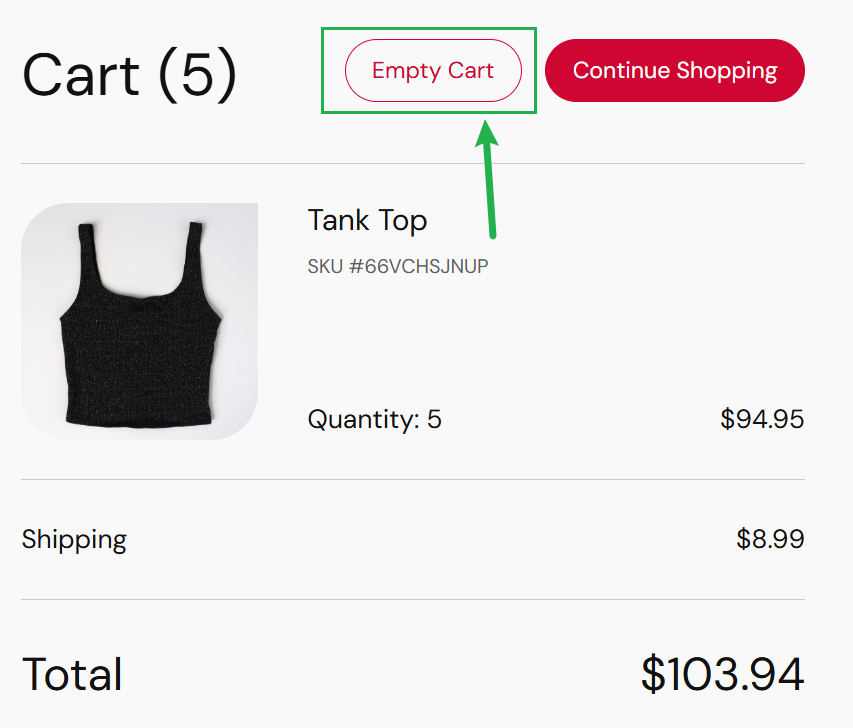
\includegraphics[width=\textwidth]{figure/microservice/emptyit.png}
		清空购物车
	\end{minipage}
	\caption{加入购物车与清空购物车操作过程}
	\label{fig:appendix_inventory_cart}
\end{figure}

\begin{figure}[htbp]
	\centering
	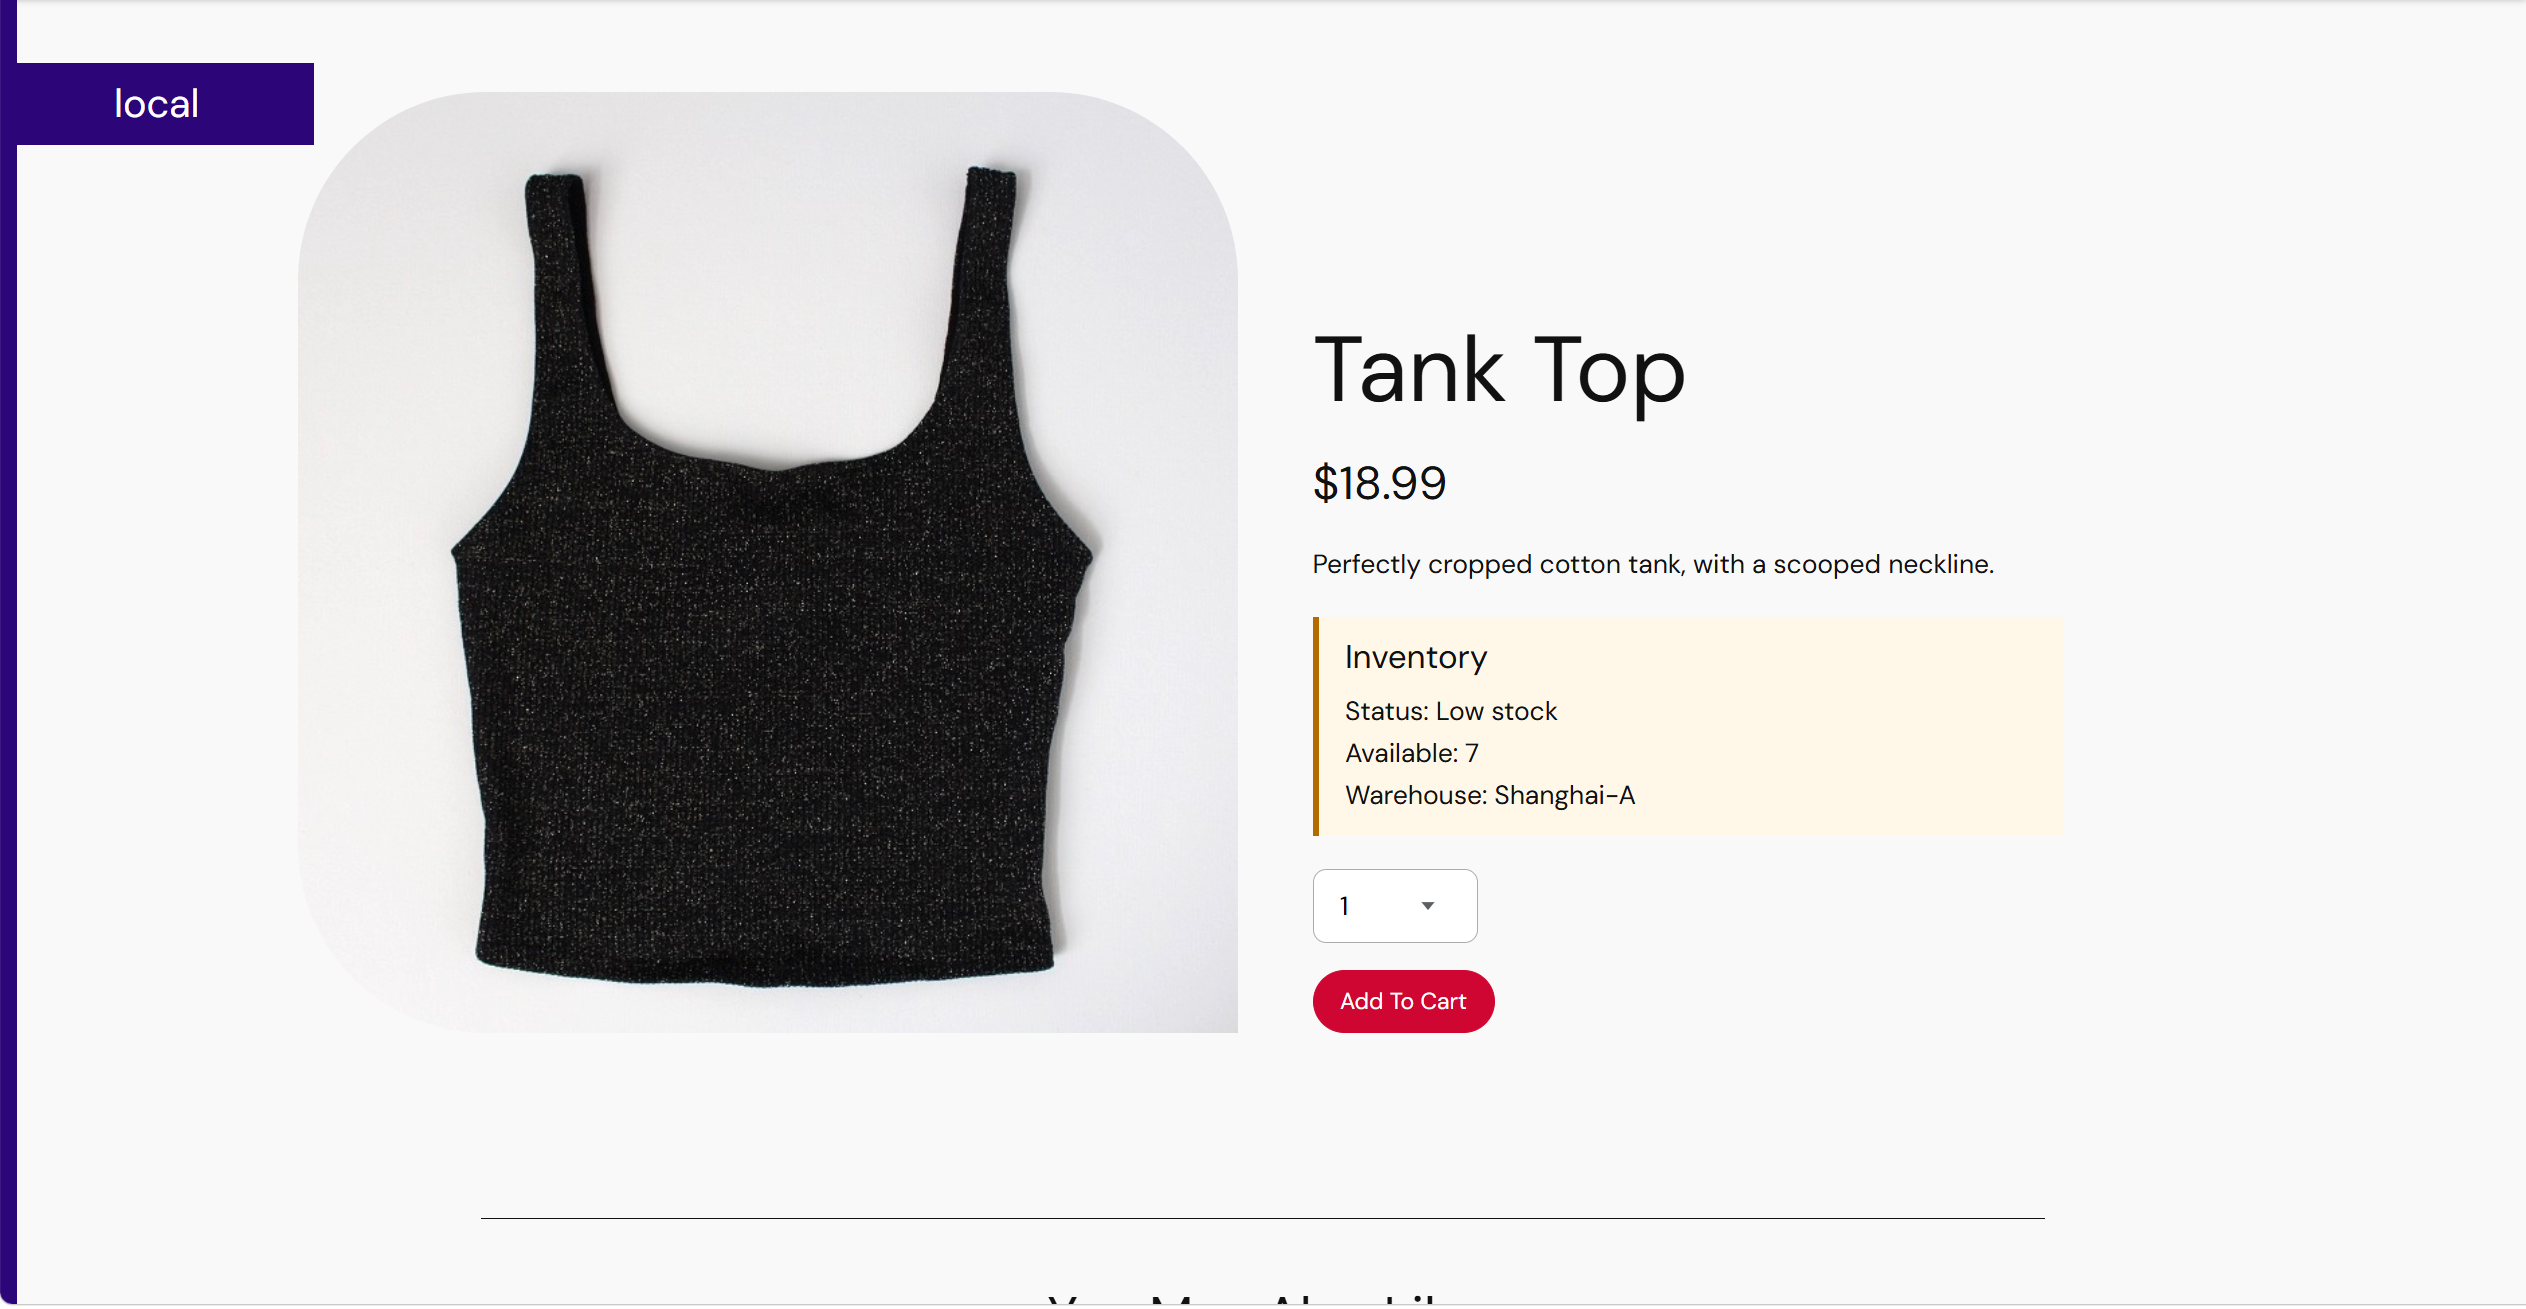
\includegraphics[width=0.85\textwidth]{figure/microservice/afteremptyit.png}
	\caption{清空购物车后库存回滚截图}
	\label{fig:appendix_inventory_after_empty}
\end{figure}

\begin{figure}[htbp]
	\centering
	\begin{minipage}{0.45\textwidth}
		\centering
		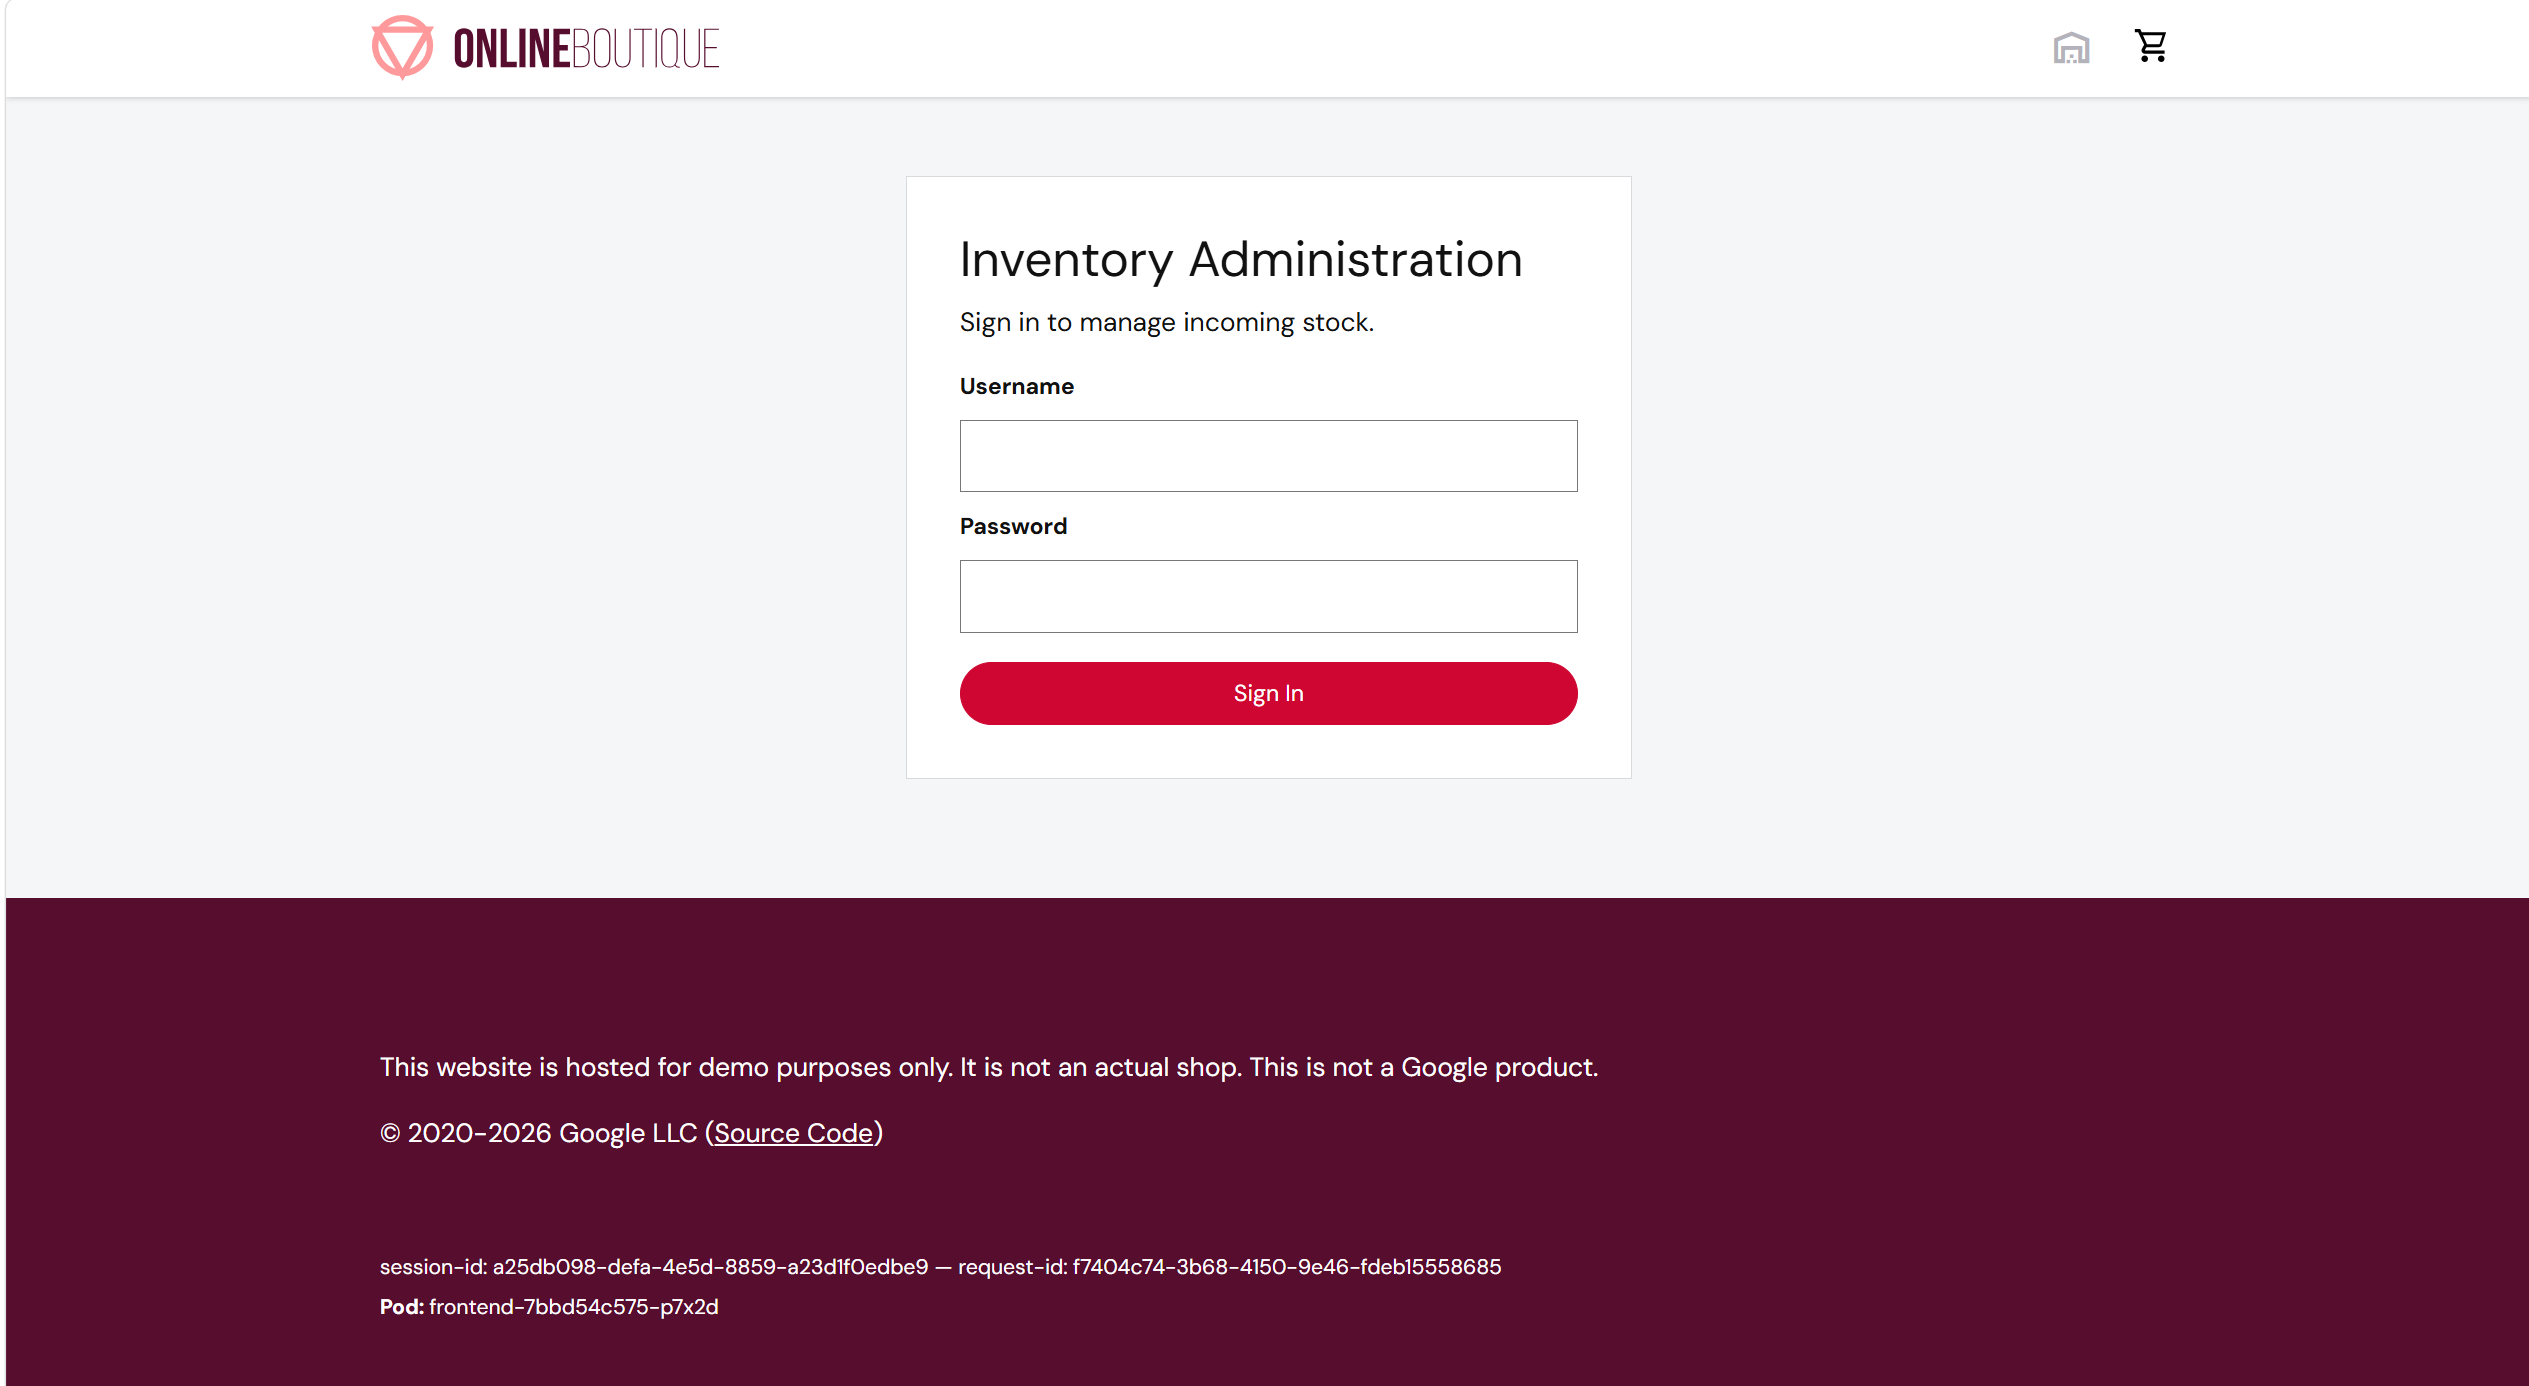
\includegraphics[width=\textwidth]{figure/microservice/inventoryadmin.png}
		管理员进货页面
	\end{minipage}
	\hfill
	\begin{minipage}{0.45\textwidth}
		\centering
		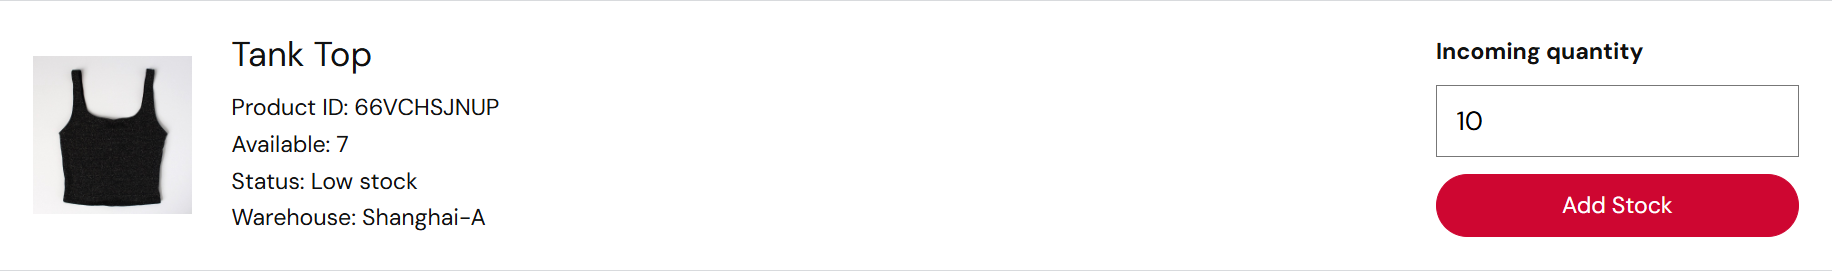
\includegraphics[width=\textwidth]{figure/microservice/inventory10.png}
		输入进货数量
	\end{minipage}
	\caption{管理员进货操作页面}
	\label{fig:appendix_restock_page}
\end{figure}

\begin{figure}[htbp]
	\centering
	\begin{minipage}{0.45\textwidth}
		\centering
		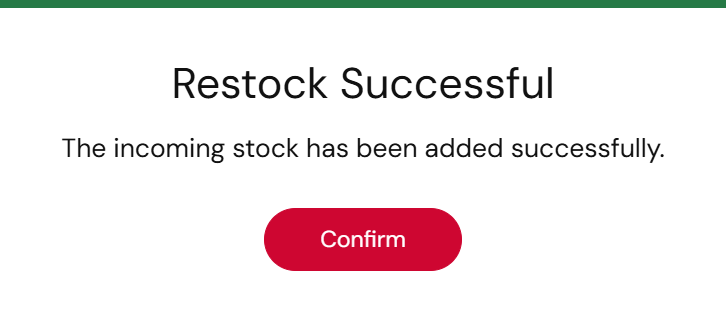
\includegraphics[width=\textwidth]{figure/microservice/respondins.png}
		进货成功弹窗
	\end{minipage}
	\hfill
	\begin{minipage}{0.45\textwidth}
		\centering
		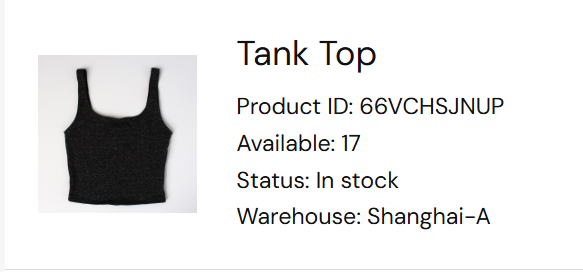
\includegraphics[width=\textwidth]{figure/microservice/avali17.png}
		进货后库存增加
	\end{minipage}
	\caption{管理员进货成功与页面刷新结果}
	\label{fig:appendix_restock_success}
\end{figure}

\begin{figure}[htbp]
	\centering
	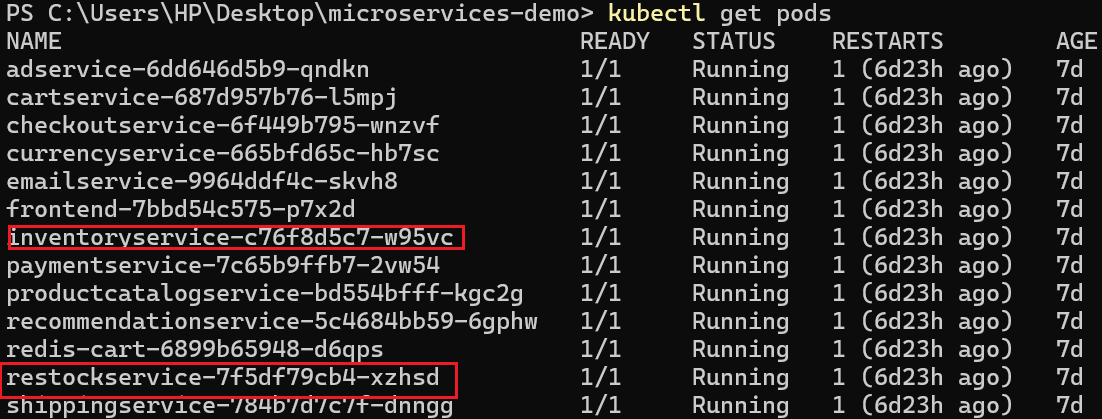
\includegraphics[width=0.85\textwidth]{figure/microservice/getpodsit.png}
	\caption{Kubernetes Pod 运行状态截图}
	\label{fig:appendix_k8s_pods}
\end{figure}

\begin{figure}[htbp]
	\centering
	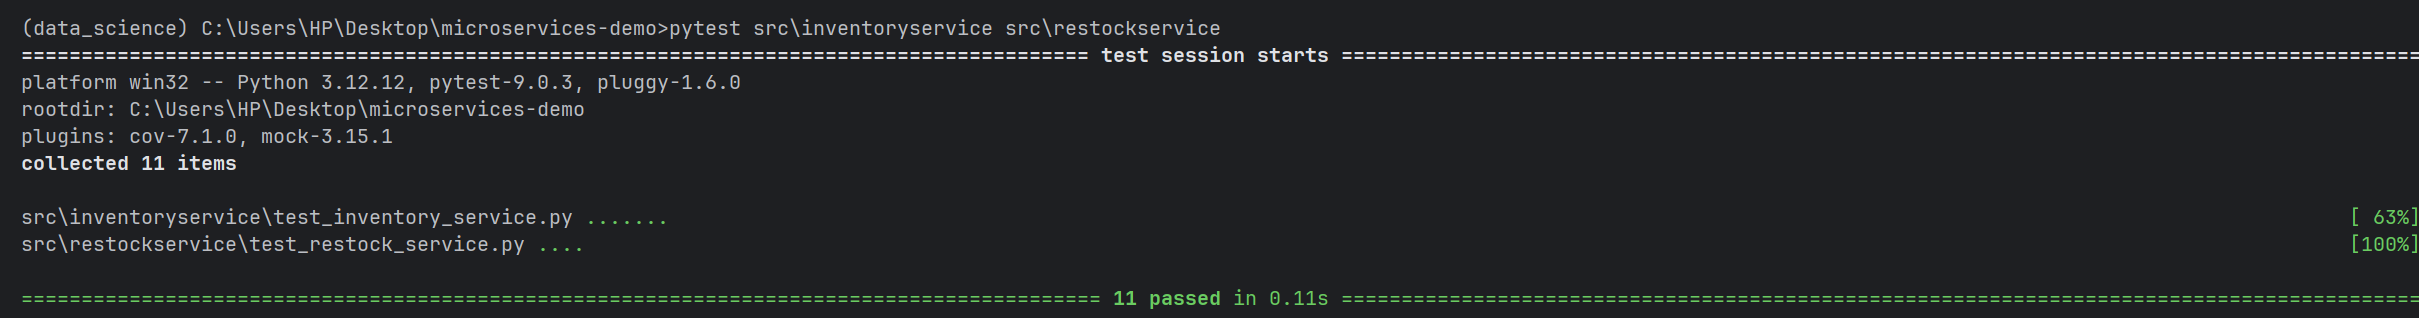
\includegraphics[width=0.85\textwidth]{figure/microservice/testitest.png}
	\caption{库存服务和进货服务单元测试通过截图}
	\label{fig:appendix_pytest}
\end{figure}


\begin{figure}[htbp]
	\centering
	
\includegraphics[width=0.8\textwidth]{"./figure/LightLog/LogRobust/training_curves.png"}
	\caption{LogRobust训练曲线}
	\label{fig:LogRobustTrain}
\end{figure}
\end{spacing}


%---------------------------------------------------------------------
%  参考文献设置
%---------------------------------------------------------------------
% \addcontentsline{toc}{chapter}{参考文献}

% \begin{thebibliography}{99}
% \songti \zihao{-4} 	
% 	\bibitem{Leslie.{1994}}
% 	Leslie Lamport. LATEX: A Document Preparation System.AddisonWesley, Reading, Massachusetts, second edition, 1994, ISBN 0-201-52983-1.
	
% 	\bibitem{Donald.{1984}}
% 	Donald E. Knuth. The TEXbook, Volume A of Computers and Typesetting,Addison Wesley, Reading, Massachusetts, second edition, 1984,ISBN 0-201-13448-9.

	
% \end{thebibliography}

%---------------------------------------------------------------------
%  附录设置
%---------------------------------------------------------------------
% \titleformat{\chapter}{\heiti\Large}{附录~\Alph{chapter}}{11pt}{\Large}
% \titlespacing{\chapter}{0pt}{*-4}{*4}

% \lstset{breaklines}                %自动将长的代码行换行排版
% \lstset{extendedchars=false}
% \lstset{language=Matlab}
% \renewcommand{\thechapter}{附录\Alph{chapter}.}
% \appendix
% \begin{appendix}
	
	

% \end{appendix}
		

\end{document}
